% Options for packages loaded elsewhere
\PassOptionsToPackage{unicode}{hyperref}
\PassOptionsToPackage{hyphens}{url}
%
\documentclass[
]{book}
\usepackage{amsmath,amssymb}
\usepackage{lmodern}
\usepackage{iftex}
\ifPDFTeX
  \usepackage[T1]{fontenc}
  \usepackage[utf8]{inputenc}
  \usepackage{textcomp} % provide euro and other symbols
\else % if luatex or xetex
  \usepackage{unicode-math}
  \defaultfontfeatures{Scale=MatchLowercase}
  \defaultfontfeatures[\rmfamily]{Ligatures=TeX,Scale=1}
\fi
% Use upquote if available, for straight quotes in verbatim environments
\IfFileExists{upquote.sty}{\usepackage{upquote}}{}
\IfFileExists{microtype.sty}{% use microtype if available
  \usepackage[]{microtype}
  \UseMicrotypeSet[protrusion]{basicmath} % disable protrusion for tt fonts
}{}
\makeatletter
\@ifundefined{KOMAClassName}{% if non-KOMA class
  \IfFileExists{parskip.sty}{%
    \usepackage{parskip}
  }{% else
    \setlength{\parindent}{0pt}
    \setlength{\parskip}{6pt plus 2pt minus 1pt}}
}{% if KOMA class
  \KOMAoptions{parskip=half}}
\makeatother
\usepackage{xcolor}
\usepackage{color}
\usepackage{fancyvrb}
\newcommand{\VerbBar}{|}
\newcommand{\VERB}{\Verb[commandchars=\\\{\}]}
\DefineVerbatimEnvironment{Highlighting}{Verbatim}{commandchars=\\\{\}}
% Add ',fontsize=\small' for more characters per line
\usepackage{framed}
\definecolor{shadecolor}{RGB}{248,248,248}
\newenvironment{Shaded}{\begin{snugshade}}{\end{snugshade}}
\newcommand{\AlertTok}[1]{\textcolor[rgb]{0.94,0.16,0.16}{#1}}
\newcommand{\AnnotationTok}[1]{\textcolor[rgb]{0.56,0.35,0.01}{\textbf{\textit{#1}}}}
\newcommand{\AttributeTok}[1]{\textcolor[rgb]{0.77,0.63,0.00}{#1}}
\newcommand{\BaseNTok}[1]{\textcolor[rgb]{0.00,0.00,0.81}{#1}}
\newcommand{\BuiltInTok}[1]{#1}
\newcommand{\CharTok}[1]{\textcolor[rgb]{0.31,0.60,0.02}{#1}}
\newcommand{\CommentTok}[1]{\textcolor[rgb]{0.56,0.35,0.01}{\textit{#1}}}
\newcommand{\CommentVarTok}[1]{\textcolor[rgb]{0.56,0.35,0.01}{\textbf{\textit{#1}}}}
\newcommand{\ConstantTok}[1]{\textcolor[rgb]{0.00,0.00,0.00}{#1}}
\newcommand{\ControlFlowTok}[1]{\textcolor[rgb]{0.13,0.29,0.53}{\textbf{#1}}}
\newcommand{\DataTypeTok}[1]{\textcolor[rgb]{0.13,0.29,0.53}{#1}}
\newcommand{\DecValTok}[1]{\textcolor[rgb]{0.00,0.00,0.81}{#1}}
\newcommand{\DocumentationTok}[1]{\textcolor[rgb]{0.56,0.35,0.01}{\textbf{\textit{#1}}}}
\newcommand{\ErrorTok}[1]{\textcolor[rgb]{0.64,0.00,0.00}{\textbf{#1}}}
\newcommand{\ExtensionTok}[1]{#1}
\newcommand{\FloatTok}[1]{\textcolor[rgb]{0.00,0.00,0.81}{#1}}
\newcommand{\FunctionTok}[1]{\textcolor[rgb]{0.00,0.00,0.00}{#1}}
\newcommand{\ImportTok}[1]{#1}
\newcommand{\InformationTok}[1]{\textcolor[rgb]{0.56,0.35,0.01}{\textbf{\textit{#1}}}}
\newcommand{\KeywordTok}[1]{\textcolor[rgb]{0.13,0.29,0.53}{\textbf{#1}}}
\newcommand{\NormalTok}[1]{#1}
\newcommand{\OperatorTok}[1]{\textcolor[rgb]{0.81,0.36,0.00}{\textbf{#1}}}
\newcommand{\OtherTok}[1]{\textcolor[rgb]{0.56,0.35,0.01}{#1}}
\newcommand{\PreprocessorTok}[1]{\textcolor[rgb]{0.56,0.35,0.01}{\textit{#1}}}
\newcommand{\RegionMarkerTok}[1]{#1}
\newcommand{\SpecialCharTok}[1]{\textcolor[rgb]{0.00,0.00,0.00}{#1}}
\newcommand{\SpecialStringTok}[1]{\textcolor[rgb]{0.31,0.60,0.02}{#1}}
\newcommand{\StringTok}[1]{\textcolor[rgb]{0.31,0.60,0.02}{#1}}
\newcommand{\VariableTok}[1]{\textcolor[rgb]{0.00,0.00,0.00}{#1}}
\newcommand{\VerbatimStringTok}[1]{\textcolor[rgb]{0.31,0.60,0.02}{#1}}
\newcommand{\WarningTok}[1]{\textcolor[rgb]{0.56,0.35,0.01}{\textbf{\textit{#1}}}}
\usepackage{longtable,booktabs,array}
\usepackage{calc} % for calculating minipage widths
% Correct order of tables after \paragraph or \subparagraph
\usepackage{etoolbox}
\makeatletter
\patchcmd\longtable{\par}{\if@noskipsec\mbox{}\fi\par}{}{}
\makeatother
% Allow footnotes in longtable head/foot
\IfFileExists{footnotehyper.sty}{\usepackage{footnotehyper}}{\usepackage{footnote}}
\makesavenoteenv{longtable}
\usepackage{graphicx}
\makeatletter
\def\maxwidth{\ifdim\Gin@nat@width>\linewidth\linewidth\else\Gin@nat@width\fi}
\def\maxheight{\ifdim\Gin@nat@height>\textheight\textheight\else\Gin@nat@height\fi}
\makeatother
% Scale images if necessary, so that they will not overflow the page
% margins by default, and it is still possible to overwrite the defaults
% using explicit options in \includegraphics[width, height, ...]{}
\setkeys{Gin}{width=\maxwidth,height=\maxheight,keepaspectratio}
% Set default figure placement to htbp
\makeatletter
\def\fps@figure{htbp}
\makeatother
\setlength{\emergencystretch}{3em} % prevent overfull lines
\providecommand{\tightlist}{%
  \setlength{\itemsep}{0pt}\setlength{\parskip}{0pt}}
\setcounter{secnumdepth}{5}
\usepackage{booktabs}
\usepackage{amsthm}
\makeatletter
\def\thm@space@setup{%
  \thm@preskip=8pt plus 2pt minus 4pt
  \thm@postskip=\thm@preskip
}
\makeatother
\ifLuaTeX
  \usepackage{selnolig}  % disable illegal ligatures
\fi
\usepackage[]{natbib}
\bibliographystyle{apalike}
\IfFileExists{bookmark.sty}{\usepackage{bookmark}}{\usepackage{hyperref}}
\IfFileExists{xurl.sty}{\usepackage{xurl}}{} % add URL line breaks if available
\urlstyle{same} % disable monospaced font for URLs
\hypersetup{
  pdftitle={Introduction to Statistics: an integrated textbook and workbook using R},
  pdfauthor={Sean Raleigh, Westminster College (Salt Lake City, UT)},
  hidelinks,
  pdfcreator={LaTeX via pandoc}}

\title{Introduction to Statistics: an integrated textbook and workbook using R}
\author{Sean Raleigh, Westminster College (Salt Lake City, UT)}
\date{2022-07-28}

\begin{document}
\maketitle

{
\setcounter{tocdepth}{1}
\tableofcontents
}
\hypertarget{intro}{%
\chapter*{Introduction}\label{intro}}
\addcontentsline{toc}{chapter}{Introduction}

Welcome to statistics!

If you want, you can also download this book as a PDF or EPUB file. Be aware that the print versions are missing some of the richer formatting of the online version. Besides, the recommended way to work through this material is to download the R notebook file (\texttt{.Rmd}) at the top of each chapter and work through it in RStudio.

\hypertarget{intro-philosophy}{%
\section*{Philosophy}\label{intro-philosophy}}
\addcontentsline{toc}{section}{Philosophy}

{[}TODO{]}

\hypertarget{intro-structure}{%
\section*{Course structure}\label{intro-structure}}
\addcontentsline{toc}{section}{Course structure}

{[}TODO{]}

\hypertarget{intro-onward}{%
\section*{Onward and upward}\label{intro-onward}}
\addcontentsline{toc}{section}{Onward and upward}

I hope you enjoy the textbook. You can provide feedback two ways:

\begin{enumerate}
\def\labelenumi{\arabic{enumi}.}
\item
  The preferred method is to file an issue on the Github page: \url{https://github.com/VectorPosse/intro_stats/issues}
\item
  Alternatively, send me an email: \href{mailto:sraleigh@westminstercollege.edu}{\nolinkurl{sraleigh@westminstercollege.edu}}
\end{enumerate}

\hypertarget{intror}{%
\chapter{Introduction to R}\label{intror}}

\hypertarget{functions-introduced-in-this-chapter}{%
\subsection*{Functions introduced in this chapter:}\label{functions-introduced-in-this-chapter}}
\addcontentsline{toc}{subsection}{Functions introduced in this chapter:}

\texttt{\textless{}-}, \texttt{c}, \texttt{sum}, \texttt{mean}, \texttt{library}, \texttt{?}, \texttt{??}, \texttt{View}, \texttt{head}, \texttt{tail}, \texttt{str}, \texttt{NROW}, \texttt{NCOL}, \texttt{summary}, \texttt{\$}

\hypertarget{intror-intro}{%
\section{Introduction}\label{intror-intro}}

Welcome to R! This chapter will walk you through everything you need to know to get started using R.

As you go through this chapter (and all future chapters), please read slowly and carefully, and pay attention to detail. Many steps depend on the correct execution of all previous steps, so reading quickly and casually might come back to bite you later.

\hypertarget{intror-whatisr}{%
\section{What is R?}\label{intror-whatisr}}

R is a programming language specifically designed for doing statistics. Don't be intimidated by the word ``programming'' though. The goal of this course is not to make you a computer programmer. To use R to do statistics, you don't need know anything about programming at all. Every chapter throughout the whole course will give you examples of the commands you need to use. All you have to do is use those example commands as templates and make the necessary changes to adapt them to the data you're trying to analyze.

The greatest thing about R is that it is free and open source. This means that you can download it and use it for free, and also that you can inspect and modify the source code for all R functions. This kind of transparency does not exist in commercial software. The net result is a robust, secure, widely-used language with literally tens of thousands of contributions from R users all over the world.

R has also become a standard tool for statistical analysis, from academia to industry to government. Although some commercial packages are still widely used, many practitioners are switching to R due to its cost (free!) and relative ease of use. After this course, you will be able to list some R experience on your résumé and your future employer will value this. It might even help get you a job!

\hypertarget{intror-rstudio}{%
\section{RStudio}\label{intror-rstudio}}

RStudio is an ``Integrated Development Environment,'\,' or IDE for short. An IDE is a tool for working with a programming language that is fancier than just a simple text editor. Most IDEs give you shortcuts, menus, debugging facilities, syntax highlighting, and other things to make your life as easy as possible.

Open RStudio so we can explore some of the areas you'll be using in the future.

On the left side of your screen, you should see a big pane called the ``Console''. There will be some startup text there, and below that, you should see a ``command prompt'': the symbol ``\textgreater{}'' followed by a blinking cursor. (If the cursor is not blinking, that means that the focus is in another pane. Click anywhere in the Console and the cursor should start blinking again.)

A command prompt can be one of the more intimidating things about starting to use R. It's just sitting there waiting for you to do something. Unlike other programs where you run commands from menus, R requires you to know what you need to type to make it work.

We'll return to the Console in a moment.

Next, look at the upper-right corner of the screen. There are at least three tabs in this pane starting with ``Environment'', ``History'', and ``Connections''. The ``Environment'' (also called the ``Global Environment'') keeps track of things you define while working with R. There's nothing to see there yet because we haven't defined anything! The ``History'' tab will likewise be empty; again, we haven't done anything yet. We won't use the ``Connections'' tab in this course. (Depending on the version of RStudio you are using and its configuration, you may see additional tabs, but we won't need them for this course.)

Now look at the lower-right corner of the screen. There are likely five tabs here: ``Files'', ``Plots'', ``Packages'', ``Help'', and ``Viewer''. The ``Files'' tab will eventually contain the files you upload or create. ``Plots'' will show you the result of commands that produce graphs and charts. ``Packages'' will be explained later. ``Help'' is precisely what it sounds like; this will be a very useful place for you to get to know. We will never use the ``Viewer'' tab, so don't worry about it.

\hypertarget{intror-trysomething}{%
\section{Try something!}\label{intror-trysomething}}

So let's do something in R! Go back to the Console and at the command prompt (the ``\textgreater{}'' symbol with the blinking cursor), type

\begin{Shaded}
\begin{Highlighting}[]
\DecValTok{1}\SpecialCharTok{+}\DecValTok{1}
\end{Highlighting}
\end{Shaded}

and hit Enter.

Congratulations! You just ran your first command in R. It's all downhill from here. R really is nothing more than a glorified calculator.

Okay, let's do something slightly more sophisticated. It's important to note that R is case-sensitive, which means that lowercase letters and uppercase letters are treated differently. Type the following, making sure you use a lowercase \texttt{c}, and hit Enter:

\begin{Shaded}
\begin{Highlighting}[]
\NormalTok{x }\OtherTok{\textless{}{-}} \FunctionTok{c}\NormalTok{(}\DecValTok{1}\NormalTok{, }\DecValTok{3}\NormalTok{, }\DecValTok{4}\NormalTok{, }\DecValTok{7}\NormalTok{, }\DecValTok{9}\NormalTok{)}
\end{Highlighting}
\end{Shaded}

You have just created a ``vector''. When we use the letter \texttt{c} and enclose a list of things in parentheses, we tell R to ``combine'' those elements. So, a vector is just a collection of data. The little arrow \texttt{\textless{}-} says to take what's on the right and assign it to the symbol on the left. The vector \texttt{x} is now saved in memory. As long as you don't terminate your current R session, this vector is available to you.

Check out the ``Environment'' pane now. You should see the vector \texttt{x} that you just created, along with some information about it. Next to \texttt{x}, it says \texttt{num}, which means your vector has numerical data. Then it says \texttt{{[}1:5{]}} which indicates that there are five elements in the vector \texttt{x}.

At the command prompt in the Console, type

\begin{Shaded}
\begin{Highlighting}[]
\NormalTok{x}
\end{Highlighting}
\end{Shaded}

and hit Enter. Yup, \texttt{x} is there. R knows what it is. You may be wondering about the \texttt{{[}1{]}} that appears at the beginning of the line. To see what that means, try typing this (and hit Enter---at some point here I'm going to stop reminding you to hit Enter after everything you type):

\begin{Shaded}
\begin{Highlighting}[]
\NormalTok{y }\OtherTok{\textless{}{-}}\NormalTok{ letters}
\end{Highlighting}
\end{Shaded}

R is clever, so the alphabet is built in under the name \texttt{letters}.

Type

\begin{Shaded}
\begin{Highlighting}[]
\NormalTok{y}
\end{Highlighting}
\end{Shaded}

Now can you see what the \texttt{{[}1{]}} meant above? Assuming the letters spilled onto more than one line of the Console, you should see a number in brackets at the beginning of each line telling you the numerical position of the first entry in each new line.

Since we've done a few things, check out the ``Global Environment'' in the upper-right corner. You should see the two objects we've defined thus far, \texttt{x} and \texttt{y}. Now click on the ``History'' tab. Here you have all the commands you have run so far. This can be handy if you need to go back and re-run an earlier command, or if you want to modify an earlier command and it's easier to edit it slightly than type it all over again. To get an older command back into the Console, either double-click on it, or select it and click the ``To Console'' button at the top of the pane.

When we want to re-use an old command, it has usually not been that long since we last used it. In this case, there is an even more handy trick. Click in the Console so that the cursor is blinking at the blank command prompt. Now hit the up arrow on your keyboard. Do it again. Now hit the down arrow once or twice. This is a great way to access the most recently used commands from your command history.

Let's do something with \texttt{x}. Type

\begin{Shaded}
\begin{Highlighting}[]
\FunctionTok{sum}\NormalTok{(x)}
\end{Highlighting}
\end{Shaded}

I bet you figured out what just happened.

Now try

\begin{Shaded}
\begin{Highlighting}[]
\FunctionTok{mean}\NormalTok{(x)}
\end{Highlighting}
\end{Shaded}

What if we wanted to save the mean of those five numbers for use later? We can assign the result to another variable! Type the following and observe the effect in the Environment.

\begin{Shaded}
\begin{Highlighting}[]
\NormalTok{m }\OtherTok{\textless{}{-}} \FunctionTok{mean}\NormalTok{(x)}
\end{Highlighting}
\end{Shaded}

It makes no difference what letter or combination of letters we use to name our variables. For example,

\begin{Shaded}
\begin{Highlighting}[]
\NormalTok{mean\_x }\OtherTok{\textless{}{-}} \FunctionTok{mean}\NormalTok{(x)}
\end{Highlighting}
\end{Shaded}

just saves the mean to a differently named variable. In general, variable names can be any combination of characters that are letters, numbers, underscore symbols (\texttt{\_}), and dots (\texttt{.}). (In this course, we will prefer underscores over dots.) You cannot use spaces or any other special character in the names of variables.\footnote{The official spec says that a valid variable name ``consists of letters, numbers and the dot or underline characters and starts with a letter or the dot not followed by a number.''} You should avoid variable names that are the same words as predefined R functions; for example, we should not type \texttt{mean\ \textless{}-\ mean(x)}.

\hypertarget{intror-loadpackages}{%
\section{Load packages}\label{intror-loadpackages}}

Packages are collections of commands, functions, and sometimes data that people all over the world write and maintain. These packages extend the capabilities of R and add useful tools. For example, we would like to use the \texttt{palmerpenguins} package because it includes an interesting data set on penguins.

If you have installed R and RStudio on your own machine instead of accessing RStudio Workbench through a browser, you'll need to type \texttt{install.packages("palmerpenguins")} if you've never used the \texttt{palmerpenguins} package before. If you are using RStudio Workbench through a browser, you may not be able to install packages because you may not have admin privileges. If you need a package that is not installed, contact the person who administers your server.

The data set is called \texttt{penguins}. Let's see what happens when we try to access this data set without loading the package that contains it. Try typing this:

\begin{Shaded}
\begin{Highlighting}[]
\NormalTok{penguins}
\end{Highlighting}
\end{Shaded}

You should have received an error. That makes sense because R doesn't know anything about a data set called \texttt{penguins}.

Now---assuming you have the \texttt{palmerpenguins} package installed---type this at the command prompt:

\begin{Shaded}
\begin{Highlighting}[]
\FunctionTok{library}\NormalTok{(palmerpenguins)}
\end{Highlighting}
\end{Shaded}

It didn't look like anything happened. However, in the background, all the stuff in the \texttt{palmerpenguins} package became available to use.

Let's test that claim. Hit the up arrow twice and get back to where you see this at the Console (or you can manually re-type it, but that's no fun!):

\begin{Shaded}
\begin{Highlighting}[]
\NormalTok{penguins}
\end{Highlighting}
\end{Shaded}

Now R knows about the \texttt{penguins} data, so the last command printed some of it to the Console.

Go look at the ``Packages'' tab in the pane in the lower-right corner of the screen. Scroll down a little until you get to the ``P''s. You should be able to find the \texttt{palmerpenguins} package. You'll also notice a check mark by it, indicating that this package is loaded into your current R session.

You must use the \texttt{library} command in every new R session in which you want to use a package.\footnote{If you have installed R and RStudio on your own machine instead of accessing RStudio Workbench through a browser, you'll want to know that \texttt{install.packages} only has to be run once, the first time you want to install a package. If you're using RStudio Workbench, you don't even need to type that because your server admin will have already done it for you.} If you terminate your R session, R forgets about the package. If you are ever in a situation where you are trying to use a command and you know you're typing it correctly, but you're still getting an error, check to see if the package containing that command has been loaded with \texttt{library}. (Many R commands are ``base R'' commands, meaning they come with R and no special package is required to access them. The set of \texttt{letters} you used above is one such example.)

\hypertarget{intror-gettinghelp}{%
\section{Getting help}\label{intror-gettinghelp}}

There are four important ways to get help with R. The first is the obvious ``Help'' tab in the lower-right pane on your screen. Click on that tab now. In the search bar at the right, type \texttt{penguins} and hit Enter. Take a few minutes to read the help file.

Help files are only as good as their authors. Fortunately, most package developers are conscientious enough to write decent help files. But don't be surprised if the help file doesn't quite tell you what you want to know. And for highly technical R functions, sometimes the help files are downright inscrutable. Try looking at the help file for the \texttt{grep} function. Can you honestly say you have any idea what this command does or how you might use it? Over time, as you become more knowledgeable about how R works, these help files get less mysterious.

The second way of getting help is from the Console. Go to the Console and type

\begin{Shaded}
\begin{Highlighting}[]
\NormalTok{?letters}
\end{Highlighting}
\end{Shaded}

The question mark tells R you need help with the R command \texttt{letters}. This will bring up the help file in the same Help pane you were looking at before.

Sometimes, you don't know exactly what the name of the command is. For example, suppose we misremembered the name and thought it was \texttt{letter} instead of \texttt{letters}. Try typing this:

\begin{Shaded}
\begin{Highlighting}[]
\NormalTok{?letter}
\end{Highlighting}
\end{Shaded}

You should have received an error because there is no command called \texttt{letter}. Try this instead:

\begin{Shaded}
\begin{Highlighting}[]
\NormalTok{??letter}
\end{Highlighting}
\end{Shaded}

and scroll down a bit in the Help pane. Two question marks tell R not to be too picky about the spelling. This will bring up a whole bunch of possibilities in the Help pane, representing R's best guess as to what you might be searching for. (In this case, it's not easy to find. You'd have to know that the help file for \texttt{letters} appeared on a help page called \texttt{base::Constants}.)

The fourth way to get help---and often the most useful way---is to use your best friend Google. You don't want to just search for ``R''. (That's the downside of using a single letter of the alphabet for the name of a programming language.) However, if you type ``R \_\_\_\_\_\_\_\_\_\_'' where you fill in the blank with the topic of interest, Google usually does a pretty good job sending you to relevant pages. Within the first few hits, in fact, you'll often see an online copy of the same help file you see in R. Frequently, the next few hits lead to \href{https://stackoverflow.com}{StackOverflow} where very knowledgeable people post very helpful responses to common questions.

Use Google to find out how to take the square root of a number in R. Test out your newly-discovered function on a few numbers to make sure it works.

\hypertarget{intror-understandingdata}{%
\section{Understanding the data}\label{intror-understandingdata}}

Let's go back to the penguins data contained in the \texttt{penguins} data set from the \texttt{palmerpenguins} package.

The first thing we do to understand a data set is to read the help file on it. (We've already done this for the \texttt{penguins} data.) Of course, this only works for data files that come with R or with a package that can be loaded into R. If you are using R to analyze your own data, presumably you don't need a help file. And if you're analyzing data from another source, you'll have to go to that source to find out about the data.

When you read the help file for \texttt{penguins}, you may have noticed that it described the ``Format'' as being ``A tibble with 344 rows and 8 variables.'' What is a ``tibble''?

The word ``tibble'' is an R-specific term that describes data organized in a specific way. A more common term is ``data frame'' (or sometimes ``data table''). The idea is that in a data frame, the rows and the columns have very specific interpretations.

Each row of a data frame represents a single object or observation. So in the \texttt{penguins} data, each row represents a penguin. If you have survey data, each row will usually represent a single person. But an ``object'' can be anything about which we collect data. State-level data might have 50 rows and each row represents an entire state.

Each column of a data frame represents a \emph{variable}, which is a property, attribute, or measurement made about the objects in the data. For example, the help file mentions that various pieces of information are recorded about each penguin, like species, bill length, flipper length, boy mass, sex, and so on. These are examples of variables. In a survey, for example, the variables will likely be the responses to individual questions.

We will use the terms tibble and data frame interchangeably in this course. They are not quite synonyms: tibbles are R-specific implementations of data frames, the latter being a more general term that applies in all statistical contexts. Nevertheless, there are no situations (at least not encountered in this course) where it makes any difference if a data set is called a tibble or a data frame.

We can also look at the data frame in ``spreadsheet'' form. Type

\begin{Shaded}
\begin{Highlighting}[]
\FunctionTok{View}\NormalTok{(penguins)}
\end{Highlighting}
\end{Shaded}

(Be sure you're using an upper-case ``V'' in \texttt{View}.) A new pane should open up in the upper-left corner of the screen. In that pane, the penguins data appears in a grid format, like a spreadsheet. The observations (individual penguins) are the rows and the variables (attributes and measurements about the penguins) are the columns. This will also let you sort each column by clicking on the arrows next to the variable name across the top.

Sometimes, we just need a little peek at the data. Try this to print just a few rows of data to the Console:

\begin{Shaded}
\begin{Highlighting}[]
\FunctionTok{head}\NormalTok{(penguins)}
\end{Highlighting}
\end{Shaded}

We can customize this by specifying the number of rows to print. (Don't forget about the up arrow trick!)

\begin{Shaded}
\begin{Highlighting}[]
\FunctionTok{head}\NormalTok{(penguins, }\AttributeTok{n =} \DecValTok{10}\NormalTok{)}
\end{Highlighting}
\end{Shaded}

The \texttt{tail} command does something similar.

\begin{Shaded}
\begin{Highlighting}[]
\FunctionTok{tail}\NormalTok{(penguins)}
\end{Highlighting}
\end{Shaded}

When we're working with HTML documents like this one, it's usually not necessary to use \texttt{View}, \texttt{head}, or \texttt{tail} because the HTML format will print the data frame a lot more neatly than it did in the Console. You do not need to type the following code; just look below it for the table that appears.

\begin{Shaded}
\begin{Highlighting}[]
\NormalTok{penguins}
\end{Highlighting}
\end{Shaded}

\begin{verbatim}
## # A tibble: 344 x 8
##    species island    bill_length_mm bill_depth_mm flipper_length_mm body_mass_g
##    <fct>   <fct>              <dbl>         <dbl>             <int>       <int>
##  1 Adelie  Torgersen           39.1          18.7               181        3750
##  2 Adelie  Torgersen           39.5          17.4               186        3800
##  3 Adelie  Torgersen           40.3          18                 195        3250
##  4 Adelie  Torgersen           NA            NA                  NA          NA
##  5 Adelie  Torgersen           36.7          19.3               193        3450
##  6 Adelie  Torgersen           39.3          20.6               190        3650
##  7 Adelie  Torgersen           38.9          17.8               181        3625
##  8 Adelie  Torgersen           39.2          19.6               195        4675
##  9 Adelie  Torgersen           34.1          18.1               193        3475
## 10 Adelie  Torgersen           42            20.2               190        4250
## # ... with 334 more rows, and 2 more variables: sex <fct>, year <int>
\end{verbatim}

You can scroll through the rows by using the numbers at the bottom or the ``Next'' button. The only thing you can't do here that you can do with \texttt{View} is sort the columns.

We want to understand the ``structure'' of our data. For this, we use the \texttt{str} command. Try it:

\begin{Shaded}
\begin{Highlighting}[]
\FunctionTok{str}\NormalTok{(penguins)}
\end{Highlighting}
\end{Shaded}

This tells us several important things. First it says that we are looking at a tibble with 344 observations of 8 variables. We can isolate those pieces of information separately as well, if needed:

\begin{Shaded}
\begin{Highlighting}[]
\FunctionTok{NROW}\NormalTok{(penguins)}
\end{Highlighting}
\end{Shaded}

\begin{Shaded}
\begin{Highlighting}[]
\FunctionTok{NCOL}\NormalTok{(penguins)}
\end{Highlighting}
\end{Shaded}

These give you the number of rows and columns, respectively.

The \texttt{str} command also tells us about each of the variables in our data set. We'll talk about these later.

We need to be able to summarize variables in the data set. The \texttt{summary} command is one way to do it:

\begin{Shaded}
\begin{Highlighting}[]
\FunctionTok{summary}\NormalTok{(penguins)}
\end{Highlighting}
\end{Shaded}

You may not recognize terms like ``Median'' or ``1st Qu.'' or ``3rd Qu.'' yet. Nevertheless, you can see why this summary could come in handy.

\hypertarget{intror-understandingvariables}{%
\section{Understanding the variables}\label{intror-understandingvariables}}

When we want to look at only one variable at a time, we use the dollar sign to grab it. Try this:

\begin{Shaded}
\begin{Highlighting}[]
\NormalTok{penguins}\SpecialCharTok{$}\NormalTok{body\_mass\_g}
\end{Highlighting}
\end{Shaded}

This will list the entire \texttt{body\_mass\_g} column, in other words, the body masses (in grams) of all the penguins in this particular study. If we only want to see the first few, we can use \texttt{head} like before.

\begin{Shaded}
\begin{Highlighting}[]
\FunctionTok{head}\NormalTok{(penguins}\SpecialCharTok{$}\NormalTok{body\_mass\_g)}
\end{Highlighting}
\end{Shaded}

If we want the structure of the variable \texttt{body\_mass\_g}, we do this:

\begin{Shaded}
\begin{Highlighting}[]
\FunctionTok{str}\NormalTok{(penguins}\SpecialCharTok{$}\NormalTok{body\_mass\_g)}
\end{Highlighting}
\end{Shaded}

Notice the letters \texttt{int} at the beginning of the line. That stands for ``integer'' which is another word for whole number. In other words, the patients' ages all appear in this data set as whole numbers. There are other data types you'll see in the future:

\begin{itemize}
\tightlist
\item
  \texttt{num}: This is for general numerical data (which can be integers as well as having decimal parts).
\item
  \texttt{chr}: This means ``character'', used for character strings, which can be any sequence of letters or numbers. For example, if the researcher recorded some notes for each penguin, these notes would be recorded in a character variable.
\item
  \texttt{factor}: This is for categorical data, which is data that groups observations together into categories. For example, \texttt{species} is categorical. These are generally recorded like character strings, but factor variables have more structure because they take on a limited number of possible values corresponding to a generally small number of categories. We'll learn a lot more about factor variables in future chapters.
\end{itemize}

There are other data types, but the ones above are by far the most common that you'll encounter on a regular basis.

If we want to summarize only the variable \texttt{body\_mass\_g}, we can do this:

\begin{Shaded}
\begin{Highlighting}[]
\FunctionTok{summary}\NormalTok{(penguins}\SpecialCharTok{$}\NormalTok{body\_mass\_g)}
\end{Highlighting}
\end{Shaded}

While executing the commands above, you may have noticed entries listed as \texttt{NA}. These are ``missing'' values. It is worth paying attention to missing values and thinking carefully about why they might be missing. For now, just make a mental note that \texttt{NA} is the code R uses for data that is missing. (This would be the same as a blank cell in a spreadsheet.)

\hypertarget{intror-projects}{%
\section{Projects}\label{intror-projects}}

Using files in R requires you to be organized. R uses what's called a ``working directory'' to find the files it needs. Therefore, you can't just put files any old place and expect R to be able to find them.

One way of ensuring that files are all located where R can find them is to organize your work into projects. Look in the far upper-right corner of the RStudio screen. You should see some text that says \texttt{Project:\ (None)}. This means we are not currently in a project. We're going to create a new project in preparation for the next chapter on using R Markdown.

Open the drop-down menu here and select \texttt{New\ Project}. When the dialog box opens, select \texttt{New\ Directory}, then \texttt{New\ Project}.

You'll need to give your project a name. In general, this should be a descriptive name---one that could still remind you in several years what the project was about. The only thing to remember is that project names and file names should not have any spaces in them. In fact, you should avoid other kinds of special characters as well, like commas, number signs, etc. Stick to letters and numerals and you should be just fine. If you want a multi-word project name or file name, I recommend using underscores. R will allow you to name projects with spaces and modern operating systems are set up to handle file names with spaces, but there are certain things that either don't work at all or require awkward workarounds when file names have spaces. In this case, let's type \texttt{intro\_stats} for the ``Directory name''. Leave everything else alone and click \texttt{Create\ Project}.

You will see the screen refresh and R will restart.

You will see a new file called \texttt{intro\_stats.Rproj} in the Files pane, but \textbf{you should never touch that file}. It's just for RStudio to keep track of your project details.

If everything works the way it should, creating a new project will create a new folder, put you in that folder, and automatically make it your working directory.

Any additional files you need for your project should be placed in this directory. In all future chapters, the first thing you will do is download the chapter file from the book website and place it here in your project folder. If you have installed R and RStudio on your own machine, you'll need to navigate your system to find the downloaded file and move or copy it to your project working directory. (This is done most easily using File Explorer in Windows and the Finder in MacOS.) If you are using RStudio Workbench through a web browser, you'll need to upload it to your project folder using the ``Upload'' button in the Files tab.

\hypertarget{intror-conclusion}{%
\section{Conclusion}\label{intror-conclusion}}

It is often said that there is a steep learning curve when learning R. This is true to some extent. R is harder to use at first than other types of software. Nevertheless, in this course, we will work hard to ease you over that first hurdle and get you moving relatively quickly. Don't get frustrated and don't give up! Learning R is worth the effort you put in. Eventually, you'll grow to appreciate the power and flexibility of R for accomplishing a huge variety of statistical tasks.

Onward and upward!

\hypertarget{rmark}{%
\chapter{Using R Markdown}\label{rmark}}

2.0

\hypertarget{functions-introduced-in-this-chapter-1}{%
\subsection*{Functions introduced in this chapter:}\label{functions-introduced-in-this-chapter-1}}
\addcontentsline{toc}{subsection}{Functions introduced in this chapter:}

No R functions are introduced here, but R Markdown syntax is explained.

\hypertarget{rmark-intro}{%
\section{Introduction}\label{rmark-intro}}

This chapter will teach you how to use R Markdown to create quality documents that incorporate text and R code seamlessly.

First, though, let's make sure you are set up in your project in RStudio.

\hypertarget{rmark-project}{%
\section{Are you in your project?}\label{rmark-project}}

If you followed the directions at the end of the last chapter, you should have created a project called \texttt{intro\_stats}. Let's make sure you're in that project.

\textbf{Look at the upper right corner of the RStudio screen. Does it say \texttt{intro\_stats}? If so, congratulations! You are in your project and you can safely skip the next paragraph and go to the next section ``Download assignment file''.}

If you're not in the \texttt{intro\_stats} project, click on whatever it does say in the upper right corner (probably \texttt{Project:\ (None)}). You can click ``Open Project'' but it's likely that the \texttt{intro\_stats} project appears in the drop-down menu in your list of recently accessed projects. So click on the project \texttt{intro\_stats}.

\hypertarget{rmark-download}{%
\section{Download the R notebook file}\label{rmark-download}}

You need to download this chapter as an R Notebook (\texttt{.Rmd}) file. Please click the following link to do so:

https://vectorposse.github.io/intro\_stats/chapter\_downloads/02-using\_r\_markdown.Rmd

The file is now likely sitting in a Downloads folder on your machine (or wherever you have set up for web files to download). If you have installed R and RStudio on your own machine, you will need to move the file from your Downloads folder into the \texttt{intro\_stats} project directory you created at the end of the last chapter. (Again, if you haven't created the \texttt{intro\_stats} project, please go back to Chapter 1 and follow the directions for doing that.) Moving files around is most easily done using File Explorer in Windows or the Finder in MacOS. If you are logged into RStudio Workbench instead, go to the Files tab and click the ``Upload'' button. From there, leave the first box alone (``Target directory''). Click the ``Choose File'' button and navigate to the folder on your machine containing the file \texttt{02\_using-r-markdown.Rmd}. Select that file and click ``OK'' to upload the file. Then you will be able to open the file in RStudio simply by clicking on it.

If you are reading this text online in the browser, be aware that there are several instructions below that won't make any sense because you're not looking at the plain text file with all the code in it. Much of the material in this book can be read and enjoyed online, but the real learning comes from downloading the chapter files (starting with Chapter 2---this one) and working through them in RStudio.

\hypertarget{rmark-whatis}{%
\section{What is R Markdown?}\label{rmark-whatis}}

The first question should really be, ``What is Markdown?''

Markdown is a way of using plain text with simple characters to indicate formatting choices in a document. For example, in a Markdown file, one can make headers by using number signs (or hashtags as the kids are calling them these days\footnote{Also called ``pound signs'' or ``octothorpes''. This is also an example of formatting a footnote!}). The notebook file itself is just a plain text file. To see the formatting, the file has to be converted to HTML, which is the format used for web pages. (This process is described below.)

R Markdown is a special version of Markdown that also allows you to include R code alongside the text. Here's an example of a ``code chunk'':

\begin{Shaded}
\begin{Highlighting}[]
\DecValTok{1} \SpecialCharTok{+} \DecValTok{1}
\end{Highlighting}
\end{Shaded}

\begin{verbatim}
## [1] 2
\end{verbatim}

Click the little dark green, right-facing arrow in the upper-right corner of the code chunk. (The icon I'm referring to is next to a faint gear icon and a lighter green icon with a downward-facing arrow.) When you ``run'' the code chunk like this, R produces output it. We'll say more about code chunks later in this document.

This document---with text and code chunks together---is called an R Notebook file.

\hypertarget{rmark-previewing}{%
\section{Previewing a document}\label{rmark-previewing}}

There is a button in the toolbar right above the text that says ``Preview''. Go ahead and push it. See what happens.

Once the pretty output is generated, take a few moments to look back and forth between it and the original R Notebook text file (the plain text in RStudio). You can see some tricks that we won't need much (embedding web links, making lists, etc.) and some tricks that we will use in every chapter (like R code chunks).

At first, you'll want to work back and forth between the R Notebook file and the HTML file to get used to how the formatting in the plain text file get translated to output in the HTML file. After a while, you will look at the HTML file less often and work mostly in the R Notebook file, only previewing when you are finished and ready to produce your final draft.

\hypertarget{rmark-literate}{%
\section{Literate programming}\label{rmark-literate}}

R Markdown is one way to implement a ``literate programming'' paradigm. The concept of literate programming was famously described by Donald Knuth, an eminent computer scientist. The idea is that computer programs should not appear in a sterile file that's full of hard-to-read, abstruse lines of computer code. Instead, functional computer code should appear interspersed with writing that explains the code.

\hypertarget{rmark-reproducible}{%
\section{Reproducible research}\label{rmark-reproducible}}

One huge benefit of organizing your work into R Notebooks is that it makes your work \emph{reproducible}. This means that anyone with access to your data and your R Notebook file should be able to re-create the exact same analysis you did.

This is a far cry from what generally happens in research. For example, if I do all my work in Microsoft Excel, I make a series of choices in how I format and analyze my data and all those choices take the form of menu commands that I point and click with my mouse. There is no record of the exact sequence of clicks that took me from point A to B all the way to Z. All I have to show for my work is the ``clean'' spreadsheet and anything I've written down or communicated about my results. If there were any errors along the way, they would be very hard to track down.\footnote{If you think these errors are trivial, Google ``Reinhart and Rogoff Excel error'\,' to read about the catastrophic consequences of seemingly trivial Excel mistakes.}

Reproducibility should be a minimum prerequisite for all statistical analysis. Sadly, that is not the case in most of the research world. We are training you to be better.

\hypertarget{rmark-structure}{%
\section{Structure of an R Notebook}\label{rmark-structure}}

Let's start from the top. Look at the very beginning of the plain R Notebook file. (If you're in RStudio, you are looking at the R Notebook file. If you are looking at the pretty HTML file, you'll need to go back to RStudio.) The section at the very top of the file that starts and ends with three hyphens is called the YAML header. (Google it if you really care why.) The title of the document appears already, but you'll need to substitute your name and today's date in the obvious places. \textbf{Scroll up and do that now.}

You've made changes to the document, so you'll need to push the ``Preview'' button again. Once that's done, look at the resulting HTML document. The YAML header has been converted into a nicely formatted document header with the new information you've provided.

Next, there is some weird looking code with instructions not to touch it. I recommend heeding that advice. This code will allow you to answer questions and have your responses appear in pretty blue boxes. In the body of the chapter, such answer boxes will be marked with tags \texttt{:::\ \{.answer\}} and \texttt{:::}. Let's try it:

Replace this text here with something else. Then preview the document and see how it appears in the HTML file.

\textbf{Be careful not to delete the two lines starting with the three colons (:::) that surround your text! If you mess this up, the rest of the document's formatting will get screwed up.}

To be clear, the colorful answer boxes are not part of the standard R Markdown tool set. That's why we had to define them manually near the top of the file. Note that the weird code itself does not show up in the HTML file. It works in the background to define the blue boxes that show up in the HTML file.

We also have section headers throughout, which in the R Notebook file look like:

\hypertarget{section-header}{%
\section*{Section header}\label{section-header}}

The hashtags are Markdown code for formatting headers. Additional hashtags will create subsections:

\hypertarget{not-quite-as-big}{%
\subsection*{Not quite as big}\label{not-quite-as-big}}

We could actually use a single number sign, but \texttt{\#} makes a header as big as the title, which is too big. Therefore, we will prefer \texttt{\#\#} for section headers and \texttt{\#\#\#} for subsections.

\textbf{You do need to make sure that there is a blank line before and after each section header.} To see why, look at the HTML document at this spot:
\#\# Is this a new section?
Do you see the problem?

Put a blank line before and after the line above that says ``Is this a new section?'' Preview one more time and make sure that the line now shows up as a proper section header.

\hypertarget{rmark-othertricks}{%
\section{Other formatting tricks}\label{rmark-othertricks}}

You can make text \emph{italic} or \textbf{bold} by using asterisks. (Don't forget to look at the HTML to see the result.)

You can make bullet-point lists. These can be made with hyphens, but you'll need to start after a blank line, then put the hyphens at the beginning of each new line, followed by a space, as follows:

\begin{itemize}
\tightlist
\item
  First item
\item
  Second item
\end{itemize}

If you want sub-items, indent at least two spaces and use a minus sign followed by a space.

\begin{itemize}
\tightlist
\item
  Item

  \begin{itemize}
  \tightlist
  \item
    Sub-item
  \item
    Sub-item
  \end{itemize}
\item
  Item
\item
  Item
\end{itemize}

Or you can make ordered lists. Just use numbers and R Markdown will do all the work for you. Sub-items work the same way as above. (Again, make sure you're starting after a blank line and that there is a space after the periods and hyphens.)

\begin{enumerate}
\def\labelenumi{\arabic{enumi}.}
\tightlist
\item
  First Item
\end{enumerate}

\begin{itemize}
\tightlist
\item
  Sub-item
\item
  Sub-item
\end{itemize}

\begin{enumerate}
\def\labelenumi{\arabic{enumi}.}
\setcounter{enumi}{1}
\tightlist
\item
  Second Item
\item
  Third Item
\end{enumerate}

We can make horizontal rules. There are lots of ways of doing this, but I prefer a bunch of asterisks in a row.

\begin{center}\rule{0.5\linewidth}{0.5pt}\end{center}

There are many more formatting tricks available. For a good resource on all R Markdown stuff, click on \href{https://www.rstudio.com/wp-content/uploads/2015/03/rmarkdown-reference.pdf}{this link} for a ``cheat sheet''. And note in the previous sentence the syntax for including hyperlinks in your document.\footnote{You can also access cheat sheets through the main Help menu in RStudio.}

\hypertarget{rmark-codechunks}{%
\section{R code chunks}\label{rmark-codechunks}}

The most powerful feature of R Markdown is the ability to do data analysis right inside the document. This is accomplished by including R code chunks. An R code chunk doesn't just show you the R code in your output file; it also runs that code and generates output that appears right below the code chunk.

An R code chunk starts with three ``backticks'' followed by the letter r enclosed in braces, and it ends with three more backticks. (The backtick is usually in the upper-left corner of your keyboard, next to the number 1 and sharing a key with the tilde \textasciitilde.)

In RStudio, click the little dark green, right-facing arrow in the upper-right corner of the code chunk below, just as you did earlier.

\begin{Shaded}
\begin{Highlighting}[]
\CommentTok{\# Here\textquotesingle{}s some sample R code}
\NormalTok{test }\OtherTok{\textless{}{-}} \FunctionTok{c}\NormalTok{(}\DecValTok{1}\NormalTok{, }\DecValTok{2}\NormalTok{, }\DecValTok{3}\NormalTok{, }\DecValTok{4}\NormalTok{)}
\FunctionTok{sum}\NormalTok{(test)}
\end{Highlighting}
\end{Shaded}

\begin{verbatim}
## [1] 10
\end{verbatim}

After pushing the dark green arrow, you should notice that the output of the R code appeared like magic. If you preview the HTML output, you should see the same output appear. If you hover your mouse over the dark green arrow, you should see the words ``Run Current Chunk''. We'll call this the Run button for short.

\textbf{We need to address something here that always confuses people new to R and R Markdown.} A number sign (aka ``hashtag'') in an R Notebook gives us headers for sections and subsections. In R, however, a number sign indicates a ``comment'' line. In the R code above, the line \texttt{\#\ Here\textquotesingle{}s\ some\ sample\ R\ code} is not executed as R code. But you can clearly see that the two lines following were executed as R code. So be careful! Number signs inside and outside R code chunks behave very differently.

Typically, the first code chunk that appears in our document will load any packages we need. We will be using a package called \texttt{tidyverse} (which is really a collection of lots of different packages) throughout the course. We load it now. Click on the Run button (the dark green, right-facing arrow) in the code chunk below.

\begin{Shaded}
\begin{Highlighting}[]
\FunctionTok{library}\NormalTok{(tidyverse)}
\end{Highlighting}
\end{Shaded}

\begin{verbatim}
## -- Attaching packages --------------------------------------- tidyverse 1.3.1 --
\end{verbatim}

\begin{verbatim}
## v ggplot2 3.3.6     v purrr   0.3.4
## v tibble  3.1.7     v dplyr   1.0.9
## v tidyr   1.2.0     v stringr 1.4.0
## v readr   2.1.2     v forcats 0.5.1
\end{verbatim}

\begin{verbatim}
## -- Conflicts ------------------------------------------ tidyverse_conflicts() --
## x dplyr::filter() masks stats::filter()
## x dplyr::lag()    masks stats::lag()
\end{verbatim}

The output here consists of a bunch of information generated when trying to load the package. These are not errors, even though one section is labeled ``Conflicts''. Usually, errors appear with the word ``Error'', so it's typically clear when something just didn't work. Also note that once you've loaded a package, you don't need to load it again until you restart your R session. For example, if you go back and try to run the code chunk above one more time, the output will disappear. That's because \texttt{tidyverse} is already loaded, so the second ``run'' doesn't actually generate output anymore.

Okay, let's do something interesting now. We'll revisit the \texttt{penguins} data set we introduced in the previous chapter. Remember, though, that this data set also lives in a package that needs to be loaded. Run the code chunk below to load the \texttt{palmerpenguins} package:

\begin{Shaded}
\begin{Highlighting}[]
\FunctionTok{library}\NormalTok{(palmerpenguins)}
\end{Highlighting}
\end{Shaded}

Let's see what happens when we try to run multiple commands in one code chunk:

\begin{Shaded}
\begin{Highlighting}[]
\FunctionTok{head}\NormalTok{(penguins)}
\end{Highlighting}
\end{Shaded}

\begin{verbatim}
## # A tibble: 6 x 8
##   species island bill_length_mm bill_depth_mm flipper_length_~ body_mass_g sex  
##   <fct>   <fct>           <dbl>         <dbl>            <int>       <int> <fct>
## 1 Adelie  Torge~           39.1          18.7              181        3750 male 
## 2 Adelie  Torge~           39.5          17.4              186        3800 fema~
## 3 Adelie  Torge~           40.3          18                195        3250 fema~
## 4 Adelie  Torge~           NA            NA                 NA          NA <NA> 
## 5 Adelie  Torge~           36.7          19.3              193        3450 fema~
## 6 Adelie  Torge~           39.3          20.6              190        3650 male 
## # ... with 1 more variable: year <int>
\end{verbatim}

\begin{Shaded}
\begin{Highlighting}[]
\FunctionTok{tail}\NormalTok{(penguins)}
\end{Highlighting}
\end{Shaded}

\begin{verbatim}
## # A tibble: 6 x 8
##   species island bill_length_mm bill_depth_mm flipper_length_~ body_mass_g sex  
##   <fct>   <fct>           <dbl>         <dbl>            <int>       <int> <fct>
## 1 Chinst~ Dream            45.7          17                195        3650 fema~
## 2 Chinst~ Dream            55.8          19.8              207        4000 male 
## 3 Chinst~ Dream            43.5          18.1              202        3400 fema~
## 4 Chinst~ Dream            49.6          18.2              193        3775 male 
## 5 Chinst~ Dream            50.8          19                210        4100 male 
## 6 Chinst~ Dream            50.2          18.7              198        3775 fema~
## # ... with 1 more variable: year <int>
\end{verbatim}

\begin{Shaded}
\begin{Highlighting}[]
\FunctionTok{str}\NormalTok{(penguins)}
\end{Highlighting}
\end{Shaded}

\begin{verbatim}
## tibble [344 x 8] (S3: tbl_df/tbl/data.frame)
##  $ species          : Factor w/ 3 levels "Adelie","Chinstrap",..: 1 1 1 1 1 1 1 1 1 1 ...
##  $ island           : Factor w/ 3 levels "Biscoe","Dream",..: 3 3 3 3 3 3 3 3 3 3 ...
##  $ bill_length_mm   : num [1:344] 39.1 39.5 40.3 NA 36.7 39.3 38.9 39.2 34.1 42 ...
##  $ bill_depth_mm    : num [1:344] 18.7 17.4 18 NA 19.3 20.6 17.8 19.6 18.1 20.2 ...
##  $ flipper_length_mm: int [1:344] 181 186 195 NA 193 190 181 195 193 190 ...
##  $ body_mass_g      : int [1:344] 3750 3800 3250 NA 3450 3650 3625 4675 3475 4250 ...
##  $ sex              : Factor w/ 2 levels "female","male": 2 1 1 NA 1 2 1 2 NA NA ...
##  $ year             : int [1:344] 2007 2007 2007 2007 2007 2007 2007 2007 2007 2007 ...
\end{verbatim}

If you're looking at this in RStudio, it's a bit of a mess. RStudio did its best to give you what you asked for, but there are three separate commands here. The first two (\texttt{head} and \texttt{tail}) print some of the data, so the first two boxes of output are tables showing you the head and the tail of the data. The next one (\texttt{str}) normally just prints some information to the Console. So RStudio gave you an R Console box with the output of this command.

If you look at the HTML file, you can see the situation isn't as bad. Each command and its corresponding output appear nicely separated there.

Nevertheless, it will be good practice and a good habit to get into to put multiple output-generating commands in their own R code chunks. Run the following code chunks and compare the output to the mess you saw above:

\begin{Shaded}
\begin{Highlighting}[]
\FunctionTok{head}\NormalTok{(penguins)}
\end{Highlighting}
\end{Shaded}

\begin{verbatim}
## # A tibble: 6 x 8
##   species island bill_length_mm bill_depth_mm flipper_length_~ body_mass_g sex  
##   <fct>   <fct>           <dbl>         <dbl>            <int>       <int> <fct>
## 1 Adelie  Torge~           39.1          18.7              181        3750 male 
## 2 Adelie  Torge~           39.5          17.4              186        3800 fema~
## 3 Adelie  Torge~           40.3          18                195        3250 fema~
## 4 Adelie  Torge~           NA            NA                 NA          NA <NA> 
## 5 Adelie  Torge~           36.7          19.3              193        3450 fema~
## 6 Adelie  Torge~           39.3          20.6              190        3650 male 
## # ... with 1 more variable: year <int>
\end{verbatim}

\begin{Shaded}
\begin{Highlighting}[]
\FunctionTok{tail}\NormalTok{(penguins)}
\end{Highlighting}
\end{Shaded}

\begin{verbatim}
## # A tibble: 6 x 8
##   species island bill_length_mm bill_depth_mm flipper_length_~ body_mass_g sex  
##   <fct>   <fct>           <dbl>         <dbl>            <int>       <int> <fct>
## 1 Chinst~ Dream            45.7          17                195        3650 fema~
## 2 Chinst~ Dream            55.8          19.8              207        4000 male 
## 3 Chinst~ Dream            43.5          18.1              202        3400 fema~
## 4 Chinst~ Dream            49.6          18.2              193        3775 male 
## 5 Chinst~ Dream            50.8          19                210        4100 male 
## 6 Chinst~ Dream            50.2          18.7              198        3775 fema~
## # ... with 1 more variable: year <int>
\end{verbatim}

\begin{Shaded}
\begin{Highlighting}[]
\FunctionTok{str}\NormalTok{(penguins)}
\end{Highlighting}
\end{Shaded}

\begin{verbatim}
## tibble [344 x 8] (S3: tbl_df/tbl/data.frame)
##  $ species          : Factor w/ 3 levels "Adelie","Chinstrap",..: 1 1 1 1 1 1 1 1 1 1 ...
##  $ island           : Factor w/ 3 levels "Biscoe","Dream",..: 3 3 3 3 3 3 3 3 3 3 ...
##  $ bill_length_mm   : num [1:344] 39.1 39.5 40.3 NA 36.7 39.3 38.9 39.2 34.1 42 ...
##  $ bill_depth_mm    : num [1:344] 18.7 17.4 18 NA 19.3 20.6 17.8 19.6 18.1 20.2 ...
##  $ flipper_length_mm: int [1:344] 181 186 195 NA 193 190 181 195 193 190 ...
##  $ body_mass_g      : int [1:344] 3750 3800 3250 NA 3450 3650 3625 4675 3475 4250 ...
##  $ sex              : Factor w/ 2 levels "female","male": 2 1 1 NA 1 2 1 2 NA NA ...
##  $ year             : int [1:344] 2007 2007 2007 2007 2007 2007 2007 2007 2007 2007 ...
\end{verbatim}

This won't look any different in the HTML file, but it sure looks a lot cleaner in RStudio.

What about the two lines of the first code chunk we ran above?

\begin{Shaded}
\begin{Highlighting}[]
\NormalTok{test }\OtherTok{\textless{}{-}} \FunctionTok{c}\NormalTok{(}\DecValTok{1}\NormalTok{, }\DecValTok{2}\NormalTok{, }\DecValTok{3}\NormalTok{, }\DecValTok{4}\NormalTok{)}
\FunctionTok{sum}\NormalTok{(test)}
\end{Highlighting}
\end{Shaded}

\begin{verbatim}
## [1] 10
\end{verbatim}

Should these two lines be separated into two code chunks? If you run it, you'll see only one piece of output. That's because the line \texttt{test\ \textless{}-\ c(1,\ 2,\ 3,\ 4)} works invisibly in the background. The vector \texttt{test} gets assigned, but no output is produced. Try it and see (push the Run button):

\begin{Shaded}
\begin{Highlighting}[]
\NormalTok{test }\OtherTok{\textless{}{-}} \FunctionTok{c}\NormalTok{(}\DecValTok{1}\NormalTok{, }\DecValTok{2}\NormalTok{, }\DecValTok{3}\NormalTok{, }\DecValTok{4}\NormalTok{)}
\end{Highlighting}
\end{Shaded}

So while there's no harm in separating these lines and putting them in their own chunks, it's not strictly necessary. You really only need to separate lines when they produce output. (And even then, if you forget, RStudio will kindly give you multiple boxes of output.)

Suppose we define a new variable called \texttt{test2} in a code chunk. FOR PURPOSES OF THIS EXERCISE, DO NOT HIT THE RUN BUTTON YET! But do go look at the HTML file.

\begin{Shaded}
\begin{Highlighting}[]
\NormalTok{test2 }\OtherTok{\textless{}{-}} \FunctionTok{c}\NormalTok{(}\StringTok{"a"}\NormalTok{, }\StringTok{"b"}\NormalTok{, }\StringTok{"c"}\NormalTok{)}
\NormalTok{test2}
\end{Highlighting}
\end{Shaded}

\begin{verbatim}
## [1] "a" "b" "c"
\end{verbatim}

The first line defines \texttt{test2} invisibly. The second line asks R to print the value of \texttt{test2}, but in the HTML file we see no output. That's because we have not run the code chunk yet. DON'T HIT THE RUN BUTTON YET!

Okay, now go to the Console in RStudio (in the lower left corner of the screen). Try typing test2. You should get an ``Error: object `test2' not found.''

Why does this happen? The Global Environment doesn't know about it yet. Look in the upper right corner of the screen, under the ``Environment'' tab. You should see \texttt{test}, but not \texttt{test2}.

Okay, NOW GO BACK AND CLICK THE RUN BUTTON IN THE LAST CHUNK ABOVE. The output appears in RStudio below the code chunk and the Global Environment has been updated.

The take home message is this:

\textbf{Be sure to run all your code chunks in RStudio!}

In RStudio, look in the toolbar above this document, toward the right. You should see the word ``Run'' with a little drop-down menu next to it. Click on that drop-down menu and select ``Run All''. Do you see what happened? All the code chunks ran again, and that means that anything in the Global Environment will now be updated to reflect the definitions made in the R Notebook.

It's a good idea to ``Run All'' when you first open a new R Notebook. This will ensure that all your code chunks have their output below them (meaning you don't have to go through and click the Run button manually for each chunk, one at a time) and the Global Environment will accurately reflect the variables you are using.

You can ``Run All'' from time to time, but it's easier just to ``Run All'' once at the beginning, and then Run individual R code chunks manually as you create them.

Now go back to the Environment tab and find the icon with the little broom on it. Click it. You will get a popup warning you that you about to ``remove all objects from the environment''. Click ``Yes''. Now the Global Environment is empty. Go back to the ``Run'' menu and select ``Run All''. All the objects you defined in the R Notebook file are back.

Clearing out your environment can be useful from time to time. Maybe you've been working on a chapter for a while and you've tried a bunch of stuff that didn't work, or you went back and changed a bunch of code. Eventually, all that junk accumulates in your Global Environment and it can mess up your R Notebook. For example, let's define a variable called \texttt{my\_variable}.

\begin{Shaded}
\begin{Highlighting}[]
\NormalTok{my\_variable }\OtherTok{\textless{}{-}} \DecValTok{42}
\end{Highlighting}
\end{Shaded}

Then, let's do some calculation with \texttt{my\_variable}.

\begin{Shaded}
\begin{Highlighting}[]
\NormalTok{my\_variable }\SpecialCharTok{*} \DecValTok{2}
\end{Highlighting}
\end{Shaded}

\begin{verbatim}
## [1] 84
\end{verbatim}

Perhaps later you decide you don't really need \texttt{my\_variable}. Put a hashtag in front of the code \texttt{my\_variable\ \textless{}-\ 42} to comment it out so that it will no longer run, but don't touch the next code chunk where you multiply it by 2. Now try running the code chunk with \texttt{my\_variable\ *\ 2} again. Note that \texttt{my\_variable} is still sitting in your Global Environment, so you don't get any error messages. R can still see and access \texttt{my\_variable}.

Now go to the ``Run'' menu and select ``Restart R and Run All Chunks''. This clears the Global Environment and runs all the R code starting from the top of the R Notebook. This time you will get an error message: \texttt{object\ \textquotesingle{}my\_variable\textquotesingle{}\ not\ found}. You've tried to calculate with a variable called \texttt{my\_variable} that doesn't exist anymore. (The line in which it was defined has been commented out.)

It's best to make sure all your code chunks will run when loaded from a clean R session. The ``Restart R and Run All Chunks'' option is an easy way to both clear your environment and re-run all code chunks. You can do this as often as you want, but you will definitely want to do this one last time when you are done. \textbf{At the end of the chapter, when you are ready to prepare the final draft, please select ``Restart R and Run All Chunks''. Make sure everything still works!}

To get rid of the error above, uncomment the line \texttt{my\_variable\ \textless{}-\ 42} by removing the hashtag you added earlier.

\hypertarget{rmark-inline}{%
\section{Inline R commands}\label{rmark-inline}}

You don't need a standalone R code chunk to do computations. One neat feature is the ability to use R to calculate things right in the middle of your text.

Here's an example. Suppose we wanted to compute the mean body mass (in grams) for the penguins in the \texttt{penguins} data set. We could do this:

\begin{Shaded}
\begin{Highlighting}[]
\FunctionTok{mean}\NormalTok{(penguins}\SpecialCharTok{$}\NormalTok{body\_mass\_g, }\AttributeTok{na.rm =} \ConstantTok{TRUE}\NormalTok{)}
\end{Highlighting}
\end{Shaded}

\begin{verbatim}
## [1] 4201.754
\end{verbatim}

(The \texttt{na.rm\ =\ TRUE} part is necessary because two of the penguins are missing body mass data. More on missing data in future chapters.)

But we can also do this inline by using backticks and putting the letter \texttt{r} inside the first backtick. Go to the HTML document to see how the following sentence appears:

The mean body mass for penguins in the \texttt{penguins} data set is 4201.754386 grams.

You can (and should) check to make sure your inline R code is working by checking the HTML output, but you don't necessarily need to go to the HTML file to find out. In RStudio, click so that the cursor is somewhere in the middle of the inline code chunk in the paragraph above. Now type Ctrl-Enter or Cmd-Enter (PC or Mac respectively). A little box should pop up that shows you the answer!

Notice that in addition to the inline R command that calculated the mean, I also enclosed \texttt{penguins} in backticks to make it stand out in the output. I'll continue to do that for all computer commands and R functions. But to be clear, putting a word in backticks is just a formatting trick. If you want inline R code, you also need the letter \texttt{r} followed by a space inside the backticks.

\hypertarget{rmark-copypaste}{%
\section{Copying and pasting}\label{rmark-copypaste}}

In future chapters, you will be shown how to run statistical analyses using R. Each chapter will give extensive explanations of the statistical concepts and demonstrations of the necessary R code. Afterwards, there will be one or more exercises that ask you to apply your new-found knowledge to run similar analyses on your own with different data.

The idea is that you should be able to copy and paste the R code from the previously worked examples. \textbf{But you must be thoughtful about how you do this.} The code cannot just be copied and pasted blindly. It must be modified so that it applies to the exercises with new data. This requires that you understand what the code is doing. You cannot effectively modify the code if you don't know which parts to modify.

There will also be exercises in which you are asked to provide your own explanations and interpretations of your analyses. These should \textbf{not} be copied and pasted from any previous work. These exercises are designed to help you understand the statistical concepts, so they must be in your own words, using your own understanding.

In order to be successful in these chapters, you must do the following:

\begin{enumerate}
\def\labelenumi{\arabic{enumi}.}
\tightlist
\item
  \textbf{Read every part of the chapter carefully!}
\end{enumerate}

\begin{itemize}
\tightlist
\item
  It will be tempting to skim over the paragraphs quickly and just jump from code chunk to code chunk. This will be highly detrimental to your ability to gain the necessary understanding---not just to complete the chapter, but to succeed in statistics overall.
\end{itemize}

\begin{enumerate}
\def\labelenumi{\arabic{enumi}.}
\setcounter{enumi}{1}
\tightlist
\item
  \textbf{Copy and paste thoughtfully!}
\end{enumerate}

\begin{itemize}
\tightlist
\item
  Not every piece of code from the early part of the chapter will necessarily apply to the later exercises. And the code that does apply will need to be modified (sometimes quite heavily) to be able to run new analyses. Your job is to understand how the code works so that you can make changes to it without breaking things. If you don't understand a piece of code, don't copy and paste it until you've read and re-read the earlier exposition that explains how the code works.
\end{itemize}

One final note about copying and pasting. Sometimes, people will try to copy and paste code from the HTML output file. This is a bad idea. The HTML document uses special characters to make the output look pretty, but these characters don't actually work as plain text in an R Notebook. The same applies to things copied and pasted from a Word document or another website. If you need to copy and paste code, be sure to find the plain text R Notebook file (the one with the .Rmd extension here in RStudio) and copy and paste from that.

\hypertarget{rmark-conclusion}{%
\section{Conclusion}\label{rmark-conclusion}}

That's it! There wasn't too much you were asked to do for this assignment that will actually show up in the HTML output. (Make sure you did do the three things that were asked of you however: one was adding your name and the date to the YAML header, one was typing something in the blue answer box, and the last was to make a section header appear properly.) As you gain confidence and as we move into more serious stats material, you will be asked to do a lot more.

\hypertarget{rmark-prep}{%
\section{Preparing and submitting your assignment}\label{rmark-prep}}

If you look in your project folder, you should see three files:

\begin{verbatim}
intro_stats.Rproj
02-using_r_markdown.Rmd
02-using_r_markdown.nb.html
\end{verbatim}

The first file (with extension \texttt{.Rproj}) you were instructed never to touch.

The next file (with extension \texttt{.Rmd}) is your R Notebook file. It's the file you're looking at right now. It is really nothing more than a plain text file, although when you open it in RStudio, some magic allows you to see the output from the code chunks you run.

Finally, you have a file with extension \texttt{.nb.html}. That is the pretty output file generated when you hit the ``Preview'' button. (If you happen to see other files in your project folder, you should ignore those and not mess with them.) This is the ``final product'' of your work.

There are several steps that you should follow at the end of each of every chapter.

\begin{enumerate}
\def\labelenumi{\arabic{enumi}.}
\tightlist
\item
  From the ``Run'' menu, select ``Restart R and Run All Chunks''.
\item
  Deal with any code errors that crop up. Repeat steps 1---2 until there are no more code errors.
\item
  Spell check your document by clicking the icon with ``ABC'' and a check mark.
\item
  Hit the ``Preview'' button one last time to generate the final draft of the \texttt{.nb.html} file.
\item
  Proofread the HTML file carefully. If there are errors, go back and fix them, then repeat steps 1--5 again.
\end{enumerate}

If you have completed this chapter as part of a statistics course, follow the directions you receive from your professor to submit your assignment.

\hypertarget{categorical}{%
\chapter{Categorical data}\label{categorical}}

2.0

\hypertarget{functions-introduced-in-this-chapter-2}{%
\subsection*{Functions introduced in this chapter:}\label{functions-introduced-in-this-chapter-2}}
\addcontentsline{toc}{subsection}{Functions introduced in this chapter:}

\texttt{glimpse}, \texttt{table}, \texttt{tabyl}, \texttt{adorn\_pct\_formatting}, \texttt{ggplot}, \texttt{geom\_bar}, \texttt{adorn\_percentages}, \texttt{mutate}, \texttt{as\_factor}, \texttt{labs}, \texttt{tibble}, \texttt{geom\_col}

\hypertarget{categorical-intro}{%
\section{Introduction}\label{categorical-intro}}

In this chapter, we'll learn about categorical data and how to summarize it using tables and graphs.

\hypertarget{categorical-download}{%
\section{Download the R notebook file}\label{categorical-download}}

Check the upper-right corner in RStudio to make sure you're in your \texttt{intro\_stats} project. Then click on the following link to download this chapter as an R notebook file (\texttt{.Rmd}).

https://vectorposse.github.io/intro\_stats/chapter\_downloads/03-categorical\_data.Rmd

Once the file is downloaded, move it to your project folder in RStudio and open it there.

\hypertarget{categorical-restart}{%
\section{Restart R and run all chunks}\label{categorical-restart}}

In RStudio, in the toolbar above this document, find the ``Run'' drop-down menu and select ``Restart R and Run All Chunks.''

This does two important things:

\begin{enumerate}
\def\labelenumi{\arabic{enumi}.}
\tightlist
\item
  R will restart. This will clear out the Global Environment and provide a fresh session for this new assignment. None of the clutter from previous chapters will be there to mess up your work in this chapter.
\item
  All the code chunks in this document will run so that you can see the output as you scroll past it. This saves you some effort in having to click the little green ``Run'' button in each code chunk as you come across it. (Also, if you forget to run one, that could cause errors later on, so this way, all the variables you need will be in the Global Environment for when they're needed later.) You will still need to click the green arrow for new code chunks that you create, of course.
\end{enumerate}

At the end of the assignment, you will ``Restart R and Run All Chunks'' once again to make sure that everything works smoothly and there are no lingering errors.

\hypertarget{categorical-load}{%
\section{Load packages}\label{categorical-load}}

We load the \texttt{tidyverse} package since it also loads the \texttt{ggplot2} package that we'll use throughout the course to make graphs. It also loads several other packages, for example, one called \texttt{dplyr} to give us a command called \texttt{mutate}, and another called \texttt{forcats} to give us \texttt{as\_factor}. (These will all be explained later.) The \texttt{janitor} package gives us the \texttt{tabyl} command for creating nice tables. Finally, We load the \texttt{palmerpenguins} package to work with the penguin data.

\begin{Shaded}
\begin{Highlighting}[]
\FunctionTok{library}\NormalTok{(tidyverse)}
\FunctionTok{library}\NormalTok{(janitor)}
\end{Highlighting}
\end{Shaded}

\begin{verbatim}
## 
## Attaching package: 'janitor'
\end{verbatim}

\begin{verbatim}
## The following objects are masked from 'package:stats':
## 
##     chisq.test, fisher.test
\end{verbatim}

\begin{Shaded}
\begin{Highlighting}[]
\FunctionTok{library}\NormalTok{(palmerpenguins)}
\end{Highlighting}
\end{Shaded}

\hypertarget{categorical-data}{%
\section{Categorical data}\label{categorical-data}}

Data comes in different types depending on what is being measured. When people think of ``data'', they often imagine \emph{numerical data}, consisting of numbers. But there are other kinds of data as well.

In this chapter, we focus on \emph{categorical data} that groups observations into categories.

For example, if we record the species of a penguin, that is not a number. It's a word that classifies that penguin into one of a finite number of types. Whenever you see words in a data set, there's a good chance that you're looking at categorical data.

Even ``numbers'' can sometimes represent categorical data. For example, suppose in a survey there is a Yes/No question. Instead of seeing the words ``Yes'' or ``No'', though, you might see a data set with ones and zeros, where 1 = Yes and 0 = No.~The presence of numbers does not automatically make that data numerical. In fact, the data is categorical. Yes and No are categories that sort the survey respondents into two groups based on their responses to a certain question.

What about ZIP codes? They are recorded as numbers, and unlike the Yes/No example above, those numbers aren't just substitutes for words. Nevertheless, ZIP codes are categorical. They sort addresses into a finite number of groups based on geographic proximity.

Another way to think of it is this: can the numerical values of ZIP codes be treated as numbers in any meaningful way? Can you take a sum or an average of ZIP codes? Sure, technically a computer can add up or average a set of ZIP codes, but would the result be a meaningful number? Since the answer is ``no'' we cannot think of ZIP codes as numbers, even though they are recorded that way.

\hypertarget{exercise-1}{%
\paragraph*{Exercise 1}\label{exercise-1}}
\addcontentsline{toc}{paragraph}{Exercise 1}

Think of another type of data that would be recorded using numbers but should be thought of as categorical data.

Please write up your answer here.

\hypertarget{categorical-factor}{%
\section{Factor variables}\label{categorical-factor}}

R uses the term ``factor variable'' to refer to a categorical variable. Look at the structure of the \texttt{penguins} data below.

\begin{Shaded}
\begin{Highlighting}[]
\FunctionTok{str}\NormalTok{(penguins)}
\end{Highlighting}
\end{Shaded}

\begin{verbatim}
## tibble [344 x 8] (S3: tbl_df/tbl/data.frame)
##  $ species          : Factor w/ 3 levels "Adelie","Chinstrap",..: 1 1 1 1 1 1 1 1 1 1 ...
##  $ island           : Factor w/ 3 levels "Biscoe","Dream",..: 3 3 3 3 3 3 3 3 3 3 ...
##  $ bill_length_mm   : num [1:344] 39.1 39.5 40.3 NA 36.7 39.3 38.9 39.2 34.1 42 ...
##  $ bill_depth_mm    : num [1:344] 18.7 17.4 18 NA 19.3 20.6 17.8 19.6 18.1 20.2 ...
##  $ flipper_length_mm: int [1:344] 181 186 195 NA 193 190 181 195 193 190 ...
##  $ body_mass_g      : int [1:344] 3750 3800 3250 NA 3450 3650 3625 4675 3475 4250 ...
##  $ sex              : Factor w/ 2 levels "female","male": 2 1 1 NA 1 2 1 2 NA NA ...
##  $ year             : int [1:344] 2007 2007 2007 2007 2007 2007 2007 2007 2007 2007 ...
\end{verbatim}

The categorical variables \texttt{species}, \texttt{island}, and \texttt{sex} are coded correctly as factor variables.

The \texttt{tidyverse} package offers a function called \texttt{glimpse} that effectively does the same thing as \texttt{str}. We'll use \texttt{glimpse} throughout the rest of the course.

\begin{Shaded}
\begin{Highlighting}[]
\FunctionTok{glimpse}\NormalTok{(penguins)}
\end{Highlighting}
\end{Shaded}

\begin{verbatim}
## Rows: 344
## Columns: 8
## $ species           <fct> Adelie, Adelie, Adelie, Adelie, Adelie, Adelie, Adel~
## $ island            <fct> Torgersen, Torgersen, Torgersen, Torgersen, Torgerse~
## $ bill_length_mm    <dbl> 39.1, 39.5, 40.3, NA, 36.7, 39.3, 38.9, 39.2, 34.1, ~
## $ bill_depth_mm     <dbl> 18.7, 17.4, 18.0, NA, 19.3, 20.6, 17.8, 19.6, 18.1, ~
## $ flipper_length_mm <int> 181, 186, 195, NA, 193, 190, 181, 195, 193, 190, 186~
## $ body_mass_g       <int> 3750, 3800, 3250, NA, 3450, 3650, 3625, 4675, 3475, ~
## $ sex               <fct> male, female, female, NA, female, male, female, male~
## $ year              <int> 2007, 2007, 2007, 2007, 2007, 2007, 2007, 2007, 2007~
\end{verbatim}

\hypertarget{exercise-2}{%
\paragraph*{Exercise 2}\label{exercise-2}}
\addcontentsline{toc}{paragraph}{Exercise 2}

Look at the output of \texttt{str} versus \texttt{glimpse} above. Write down any advantages or disadvantages you see using one versus the other. (You may also want to check the help file for the two commands to see if they offer any clues as to why you might use one over the other.)

Please write up your answer here.

\begin{center}\rule{0.5\linewidth}{0.5pt}\end{center}

Your data set may already come with its variables coded correctly as factor variables, but often they are not. As described above, numbers are often used to represent categories, so R may think that those variables represent numerical data. Later, we'll see an example of this and learn how to handle categorical variables that are not coded as factor variables in R.

\hypertarget{categorical-summarizing-one}{%
\section{Summarizing one categorical variable}\label{categorical-summarizing-one}}

If you need to summarize a single categorical variable, a \emph{frequency table} usually suffices. This is simply a table that counts up all the instances of each category. The word ``frequency'' is synonymous here with the word ``count''.

We can use the \texttt{table} command:

\begin{Shaded}
\begin{Highlighting}[]
\FunctionTok{table}\NormalTok{(penguins}\SpecialCharTok{$}\NormalTok{species)}
\end{Highlighting}
\end{Shaded}

\begin{verbatim}
## 
##    Adelie Chinstrap    Gentoo 
##       152        68       124
\end{verbatim}

Recall that the dollar sign means to grab the variable \texttt{species} from the tibble \texttt{penguins}.

You can also generate a \emph{relative frequency table} which is a table that uses proportions or percentages instead of counts.

\textbf{NOTE:} For purposes of this course, we're going to be very careful about the terms \emph{proportion} and \emph{percentage}. For us, a proportion will always be a number between 0 and 1 whereas a percentage will be between 0 and 100. Calculating a percentage is the same as multiplying a proportion by 100.

The \texttt{table} command stops being convenient if you want proportions instead of counts. Instead, we will use the \texttt{tabyl} command from the \texttt{janitor} package that was loaded near the top of the chapter. The syntax for this command is a little different. The tibble goes first, followed by a comma, followed by the variable you want to summarize:

\begin{Shaded}
\begin{Highlighting}[]
\FunctionTok{tabyl}\NormalTok{(penguins, species)}
\end{Highlighting}
\end{Shaded}

\begin{verbatim}
##    species   n   percent
##     Adelie 152 0.4418605
##  Chinstrap  68 0.1976744
##     Gentoo 124 0.3604651
\end{verbatim}

Now you get both counts and proportions. Note that in the output above, it's a little misleading to call the last column ``percent''. These are actually proportions, and we would have to multiply by 100 to get percentages.

If you really want percentages, we can use an \texttt{adorn} function to get them as follows:

\begin{Shaded}
\begin{Highlighting}[]
\FunctionTok{tabyl}\NormalTok{(penguins, species) }\SpecialCharTok{\%\textgreater{}\%}
    \FunctionTok{adorn\_pct\_formatting}\NormalTok{()}
\end{Highlighting}
\end{Shaded}

\begin{verbatim}
##    species   n percent
##     Adelie 152   44.2%
##  Chinstrap  68   19.8%
##     Gentoo 124   36.0%
\end{verbatim}

The syntax above looks a little confusing with the unusual \texttt{\%\textgreater{}\%} there. You will learn more about that weird set of symbols in a later chapter. For now, you can just copy and paste this code and make any necessary changes to the tibble and/or variables names as needed.

\hypertarget{exercise-3a}{%
\paragraph*{Exercise 3(a)}\label{exercise-3a}}
\addcontentsline{toc}{paragraph}{Exercise 3(a)}

Use the \texttt{tabyl} command as above to create a frequency table for the sex of the penguins. (You will also get a relative frequency table for free.)

\begin{Shaded}
\begin{Highlighting}[]
\CommentTok{\# Add code here to create a frequency table for sex}
\end{Highlighting}
\end{Shaded}

\hypertarget{exercise-3b}{%
\paragraph*{Exercise 3(b)}\label{exercise-3b}}
\addcontentsline{toc}{paragraph}{Exercise 3(b)}

In the table for sex that you just created, what does the last row mean?

Please write up your answer here.

\hypertarget{exercise-3c}{%
\paragraph*{Exercise 3(c)}\label{exercise-3c}}
\addcontentsline{toc}{paragraph}{Exercise 3(c)}

Now create a relative frequency table for sex that reports percentages and not proportions.

\begin{Shaded}
\begin{Highlighting}[]
\CommentTok{\# Add code here that reports percentages instead of proportions}
\end{Highlighting}
\end{Shaded}

\hypertarget{exercise-3d}{%
\paragraph*{Exercise 3(d)}\label{exercise-3d}}
\addcontentsline{toc}{paragraph}{Exercise 3(d)}

In the previous tables, what is the difference between \texttt{percent} and \texttt{valid\_percent}? Why are there two different sets of percentages being computed?

Please write up your answer here.

\hypertarget{categorical-graphing-one}{%
\section{Graphing one categorical variable}\label{categorical-graphing-one}}

When asked, ``What type of graph should I use when graphing a single categorical variable?'' the simple answer is ``None.'' If you do need to summarize a categorical variable, a frequency table usually suffices.

If you really, really want a graph, the standard type is a bar chart. But before we can create one, we need to start learning about the very important tool we will use throughout the course for graphing. It's called \texttt{ggplot} and it's part of a package called \texttt{ggplot2}.\footnote{Why the ``2''? It's a long story. Google it if you're interested in the history of the development of the \texttt{ggplot2} package.}

We don't have to load the \texttt{ggplot2} package explicitly because it got loaded alongside a number of other packages when we called \texttt{library(tidyverse)} early on in the chapter.

\hypertarget{categorical-ggplot}{%
\section{ggplot}\label{categorical-ggplot}}

The \texttt{ggplot} command is an all-purpose graphing utility. It uses a graphing philosophy derived from a book called \emph{The Grammar of Graphics} by Leland Wilkinson. The basic idea is that each variable you want to plot should correspond to some element or ``aesthetic'' component of the graph. The obvious places for data to go are along the y-axis or x-axis, but other aesthetics are important too; graphs often use color, shape, or size to illustrate different aspects of data. Once these aesthetics have been defined, we will add ``layers'' to the graph. These are objects like dots, boxes, lines, or bars that dictate the type of graph we want to see.

In an introductory course, we won't get too fancy with these graphs. But be aware that there's a whole field of data visualization that studies clear and interesting ways to understand data graphically.

It will be easier to explain the \texttt{ggplot} syntax in the context of specific graph types, so let's create a bar chart for species.

\begin{Shaded}
\begin{Highlighting}[]
\FunctionTok{ggplot}\NormalTok{(penguins, }\FunctionTok{aes}\NormalTok{(}\AttributeTok{x =}\NormalTok{ species)) }\SpecialCharTok{+}
    \FunctionTok{geom\_bar}\NormalTok{()}
\end{Highlighting}
\end{Shaded}

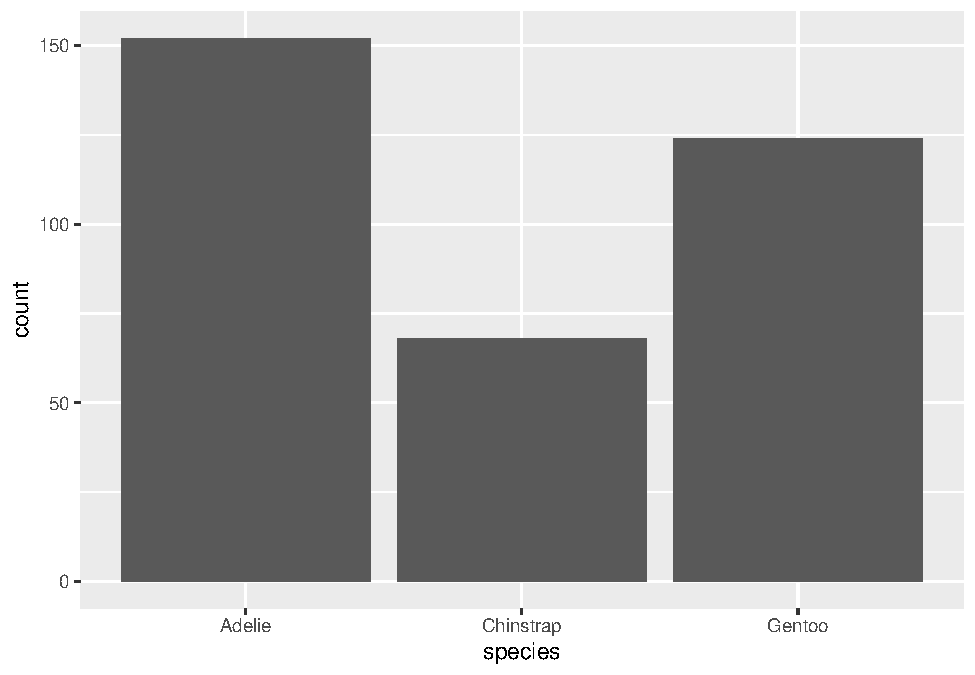
\includegraphics{intro_stats_files/figure-latex/unnamed-chunk-53-1.pdf}

We'll walk through this syntax step by step.

\begin{itemize}
\tightlist
\item
  The first argument of the \texttt{ggplot} command is the name of the tibble, in this case, \texttt{penguins}.
\item
  Next we define the aesthetics using \texttt{aes} and parentheses. Inside the parentheses, we assign any variables we want to plot to aesthetics of the graph. For this analysis, we are only interested in the variable \texttt{species} and for a bar chart, the categorical variable typically goes on the x-axis. That's why it says \texttt{x\ =\ species} inside the \texttt{aes} argument.
\item
  Finally, \texttt{ggplot} needs to know what kind of graph we want. Graph types are called ``geoms'' in the \texttt{ggplot} world, and \texttt{geom\_bar()} tells \texttt{ggplot} to add a ``bar chart layer''. Adding a layer is accomplished by literally typing a plus sign.
\end{itemize}

This can be modified somewhat to give proportions (relative frequencies) on the y-axis instead of counts. Unfortunately, the \texttt{ggplot} syntax is not very transparent here. My recommendation is to copy and paste the code below if you need to make a relative frequency bar chart in the future, making the necessary changes to the tibble and variable names, of course.

\begin{Shaded}
\begin{Highlighting}[]
\FunctionTok{ggplot}\NormalTok{(penguins, }\FunctionTok{aes}\NormalTok{(}\AttributeTok{x =}\NormalTok{ species, }\AttributeTok{y =}\NormalTok{ ..prop.., }\AttributeTok{group =} \DecValTok{1}\NormalTok{)) }\SpecialCharTok{+}
    \FunctionTok{geom\_bar}\NormalTok{()}
\end{Highlighting}
\end{Shaded}

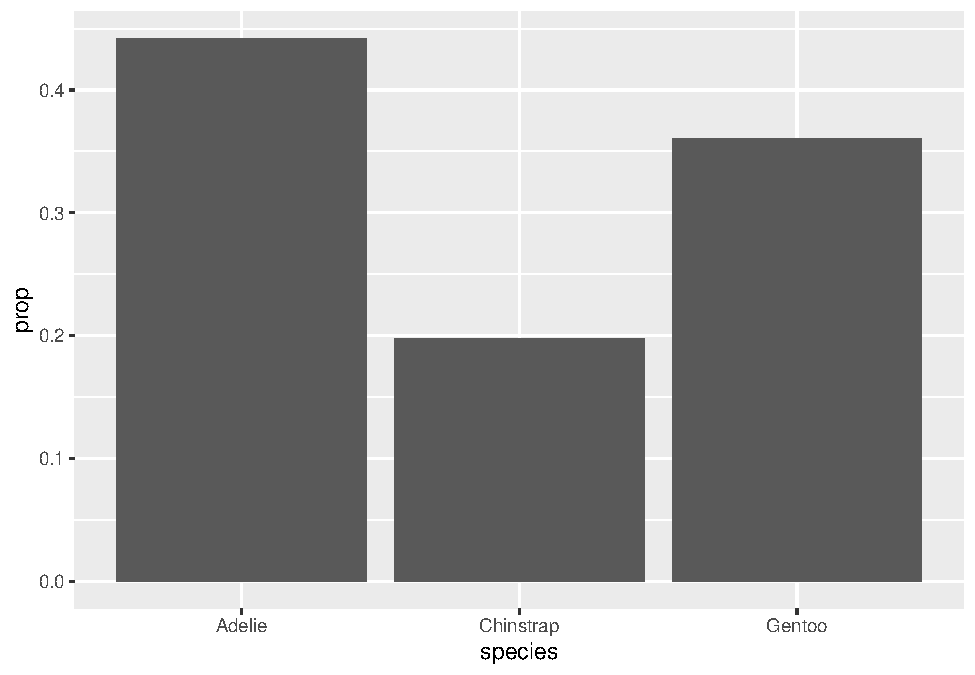
\includegraphics{intro_stats_files/figure-latex/unnamed-chunk-54-1.pdf}

These bar charts are the graphical analogues of a frequency table and a relative frequency table, respectively.

\hypertarget{exercise-4}{%
\paragraph*{Exercise 4}\label{exercise-4}}
\addcontentsline{toc}{paragraph}{Exercise 4}

In a sentence or two at most, describe the distribution of species in this data set.

Please write up your answer here.

\begin{center}\rule{0.5\linewidth}{0.5pt}\end{center}

What about pie charts? Just. Don't.

Seriously. Pie charts suck.\footnote{\url{https://medium.com/the-mission/to-pie-charts-3b1f57bcb34a}}

\hypertarget{categorical-summarizing-two}{%
\section{Summarizing two categorical variables}\label{categorical-summarizing-two}}

A table summarizing two categorical variables is called a \emph{contingency table} (or pivot table, or cross-tabulation, or probably several other terms as well).

For example, we might pose the following question: is the distribution of sex among penguins in our data more or less balanced across the three species?

When we work with two variables, typically we think of one variable as \emph{response} and the other as \emph{predictor}. The response variable is usually the variable of main interest. A predictor variable is another attribute that might predict or explain more about the response variable.

For example, our question is concerned with the sex distribution of penguins. We could create a relative frequency table of sex alone to see if male and female penguins are balanced in the data. In fact, you did that very thing above and saw that, indeed, there were roughly equal numbers of male and female penguins. But is that still true when we divide up the data into the three groups representing the separate species?

Two variables are called \emph{associated} when there is a relationship between them. For example, if sex and species were associated, then the distribution of sex would change depending on the species. Maybe one species of penguin had more females and another had fewer females. Our prediction of the sex distribution would change based on the value of the predictor variable \texttt{species}.

On the other hand, two variables that are not associated are called \emph{independent}. Independent variables are not related. If the sex distribution were the same across all species, then knowledge of the species would not change our predictions about the sex of a penguin. It wouldn't matter because there was no relationship between sex and species.

Most research questions that involve two or more variables are fundamentally questions of whether a response variable is associated with one or more predictor variables, or whether they are independent.

Let's check the contingency table. The \texttt{tabyl} command will place the first variable listed across the rows and the second one listed down the columns. It doesn't make any difference which variable is where, but to have a consistent rule on which we can rely, \textbf{let's always list the response variable first}.

\begin{Shaded}
\begin{Highlighting}[]
\FunctionTok{tabyl}\NormalTok{(penguins, sex, species)}
\end{Highlighting}
\end{Shaded}

\begin{verbatim}
##     sex Adelie Chinstrap Gentoo
##  female     73        34     58
##    male     73        34     61
##    <NA>      6         0      5
\end{verbatim}

Each column is a group, and our question is whether the distribution of sexes in each column is similar.

\hypertarget{exercise-5}{%
\paragraph*{Exercise 5}\label{exercise-5}}
\addcontentsline{toc}{paragraph}{Exercise 5}

Counts can be misleading. For example, there are 73 female Adelie penguins, but only 34 female Chinstrap penguins. Does that mean that Adelie penguins are more likely to be female than Chinstrap penguins? Why or why not?

Please write up your answer here.

\begin{center}\rule{0.5\linewidth}{0.5pt}\end{center}

A more fair way to compare across columns is to create relative frequencies. We can do this with a slightly different \texttt{adorn} command. The following code says that we want to compute column proportions (yes, I know the command is called \texttt{adorn\_percentages}, but these are proportions):

\begin{Shaded}
\begin{Highlighting}[]
\FunctionTok{tabyl}\NormalTok{(penguins, sex, species) }\SpecialCharTok{\%\textgreater{}\%}
    \FunctionTok{adorn\_percentages}\NormalTok{(}\StringTok{"col"}\NormalTok{)}
\end{Highlighting}
\end{Shaded}

\begin{verbatim}
##     sex     Adelie Chinstrap     Gentoo
##  female 0.48026316       0.5 0.46774194
##    male 0.48026316       0.5 0.49193548
##    <NA> 0.03947368       0.0 0.04032258
\end{verbatim}

If we actually want percentages, we need one more line of code. This command---\texttt{adorn\_pct\_formatting}---is the same as we used before with frequency tables.

\begin{Shaded}
\begin{Highlighting}[]
\FunctionTok{tabyl}\NormalTok{(penguins, sex, species) }\SpecialCharTok{\%\textgreater{}\%}
    \FunctionTok{adorn\_percentages}\NormalTok{(}\StringTok{"col"}\NormalTok{) }\SpecialCharTok{\%\textgreater{}\%}
    \FunctionTok{adorn\_pct\_formatting}\NormalTok{()}
\end{Highlighting}
\end{Shaded}

\begin{verbatim}
##     sex Adelie Chinstrap Gentoo
##  female  48.0%     50.0%  46.8%
##    male  48.0%     50.0%  49.2%
##    <NA>   3.9%      0.0%   4.0%
\end{verbatim}

Now we can see that each column adds up to 100\%. In other words, each species is now on equal footing, and only the distribution of sexes within each group matters.

\hypertarget{exercise-6a}{%
\paragraph*{Exercise 6(a)}\label{exercise-6a}}
\addcontentsline{toc}{paragraph}{Exercise 6(a)}

What percentage of Adelie penguins are male? What percentage of Chinstrap penguins are male? What percentage of Gentoo penguins are male?

Please write up your answer here.

\hypertarget{exercise-6b}{%
\paragraph*{Exercise 6(b)}\label{exercise-6b}}
\addcontentsline{toc}{paragraph}{Exercise 6(b)}

Does sex appear to be associated with species for the penguins in this data set? Or are these variables independent?

Please write up your answer here.

\begin{center}\rule{0.5\linewidth}{0.5pt}\end{center}

The islands of Antarctica on which the penguins were observed and measured are recorded in the variable called \texttt{island}. Is the distribution of the three species of penguin the same (or similar) on the three islands?

\hypertarget{exercise-7a}{%
\paragraph*{Exercise 7(a)}\label{exercise-7a}}
\addcontentsline{toc}{paragraph}{Exercise 7(a)}

Choosing which variables play the roles of response and predictor can be tricky. For the question above, with \texttt{species} and \texttt{island}, which is response and which is predictor?

One way to think about this is to ask the following two questions and see which one is closer to the question asked:

\begin{itemize}
\tightlist
\item
  Given information about the species, are you interested in which island the penguin lives on? If so, \texttt{species} is a predictor and \texttt{island} is response. (You are using \texttt{species} to predict \texttt{island}.)
\item
  Given information about the island, are you interested in the species of the penguin? If so, \texttt{island} is a predictor and \texttt{species} is response. (You are using \texttt{island} to predict \texttt{species}.)
\end{itemize}

Please write up your answer here.

\hypertarget{exercise-7b}{%
\paragraph*{Exercise 7(b)}\label{exercise-7b}}
\addcontentsline{toc}{paragraph}{Exercise 7(b)}

Create a contingency table with percentages. List \texttt{species} first, followed by \texttt{island}. (Hey, that's hint in case you need to go back and change your answer to part (a).)

\begin{Shaded}
\begin{Highlighting}[]
\CommentTok{\# Add code here to create a contingency table with percentages.}
\end{Highlighting}
\end{Shaded}

\hypertarget{exercise-7c}{%
\paragraph*{Exercise 7(c)}\label{exercise-7c}}
\addcontentsline{toc}{paragraph}{Exercise 7(c)}

Finally, comment on the association or independence of the two variables.

Please write up your answer here.

\hypertarget{categorical-graphing-two}{%
\section{Graphing two categorical variables}\label{categorical-graphing-two}}

A somewhat effective way to display two categorical variables is with a side-by-side bar chart. Here is the \texttt{ggplot} code for the relationship between \texttt{sex} and \texttt{species}.

\begin{Shaded}
\begin{Highlighting}[]
\FunctionTok{ggplot}\NormalTok{(penguins, }\FunctionTok{aes}\NormalTok{(}\AttributeTok{fill =}\NormalTok{ sex, }\AttributeTok{x =}\NormalTok{ species)) }\SpecialCharTok{+}
    \FunctionTok{geom\_bar}\NormalTok{(}\AttributeTok{position =} \StringTok{"dodge"}\NormalTok{)}
\end{Highlighting}
\end{Shaded}

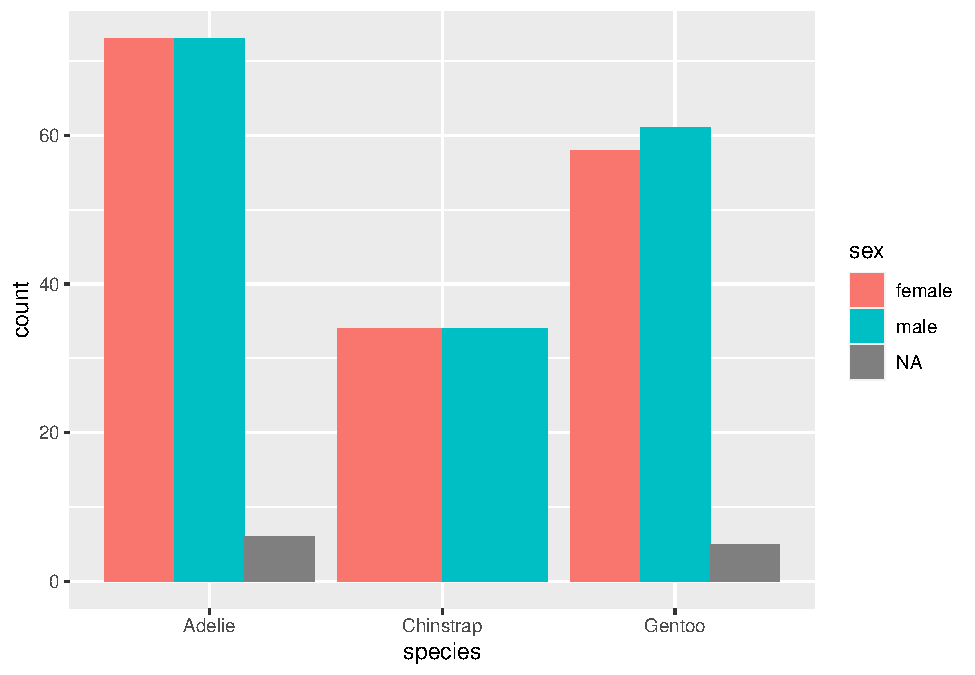
\includegraphics{intro_stats_files/figure-latex/unnamed-chunk-59-1.pdf}

This is somewhat different from the first \texttt{ggplot} example you saw above, so let's take a moment to go through it.

\begin{itemize}
\tightlist
\item
  The first argument is the data frame \texttt{penguins}; no mystery there.
\item
  The second aesthetic \texttt{x\ =\ species} also makes a lot of sense. As \texttt{species} is our predictor variable---we're using species to group the penguins, and then within each species, we're interested in the sex distribution---\texttt{species} goes on the x-axis.
\item
  However, \texttt{sex} does not go on the y-axis! (This is a very common mistake for novices.) The y-axis of a bar chart is always a count or a proportion/percentage, so no variable should ever go on the y-axis of a bar chart. In that case, how does \texttt{sex} enter the picture? Through the use of color! The aesthetic \texttt{fill\ =\ sex} says to use the \texttt{sex} variable to shade or ``fill'' the bars with different colors. You'll also notice that \texttt{ggplot} makes a legend automatically with the colors so you can see which color corresponds to which value (in this case, ``female'', ``male'', or ``NA'' for the missing data).
\end{itemize}

Another unusual feature is the argument \texttt{position\ =\ "dodge"} in the \texttt{geom\_bar} layer. Let's see what happens if we remove it.

\begin{Shaded}
\begin{Highlighting}[]
\FunctionTok{ggplot}\NormalTok{(penguins, }\FunctionTok{aes}\NormalTok{(}\AttributeTok{fill =}\NormalTok{ sex, }\AttributeTok{x =}\NormalTok{ species)) }\SpecialCharTok{+} 
    \FunctionTok{geom\_bar}\NormalTok{()}
\end{Highlighting}
\end{Shaded}

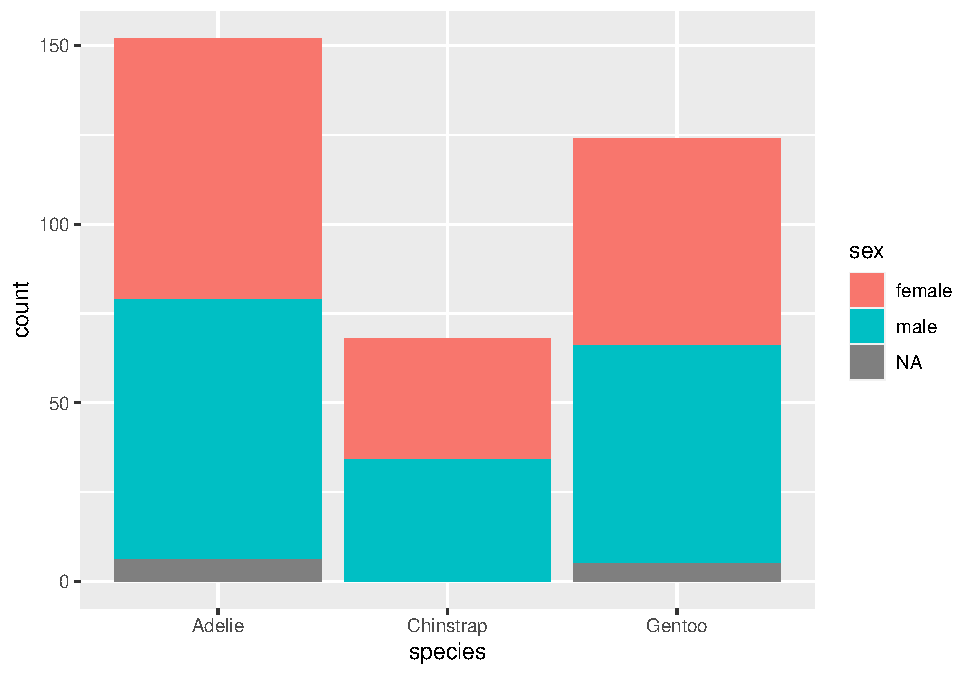
\includegraphics{intro_stats_files/figure-latex/unnamed-chunk-60-1.pdf}

We get a stacked bar chart! This is another popular way of displaying two categorical variables, but we don't tend to prefer it. Notice how difficult it is to compare the number of females across species; since there is no common baseline for the red segments of each bar, it is harder to determine which ones are bigger or smaller. (In this case, it's fairly clear, but there are plenty of data sets for which the counts might be a lot closer.)

So let's agree to use side-by-side bar charts. There is still one aspect of the side-by-side bar chart that is misleading, though. For example, the red bar for Adelie penguins is bigger than the red bar for Gentoo penguins. Does this mean Adelie penguins are more likely to be female?

This is the same issue we identified in an exercise above. To fix this problem, a better option here would be to use relative frequencies (i.e., proportions/percentages within each group) instead of counts on the y-axis. This is analogous to using proportions/percentages in a contingency table. Unfortunately, it is rather difficult to do this with \texttt{ggplot}. A compromise is available: by using \texttt{position\ =\ fill}, you can create a stacked bar chart that scales every group to 100\%. Making comparisons across groups can still be hard, as explained above for any kind of stacked bar chart, but it works okay if there are only two categories in the response variable (as is almost the case with \texttt{sex} here, although the missing data distorts things a little at the bottom).

\begin{Shaded}
\begin{Highlighting}[]
\FunctionTok{ggplot}\NormalTok{(penguins, }\FunctionTok{aes}\NormalTok{(}\AttributeTok{fill =}\NormalTok{ sex, }\AttributeTok{x =}\NormalTok{ species)) }\SpecialCharTok{+}
    \FunctionTok{geom\_bar}\NormalTok{(}\AttributeTok{position =} \StringTok{"fill"}\NormalTok{)}
\end{Highlighting}
\end{Shaded}

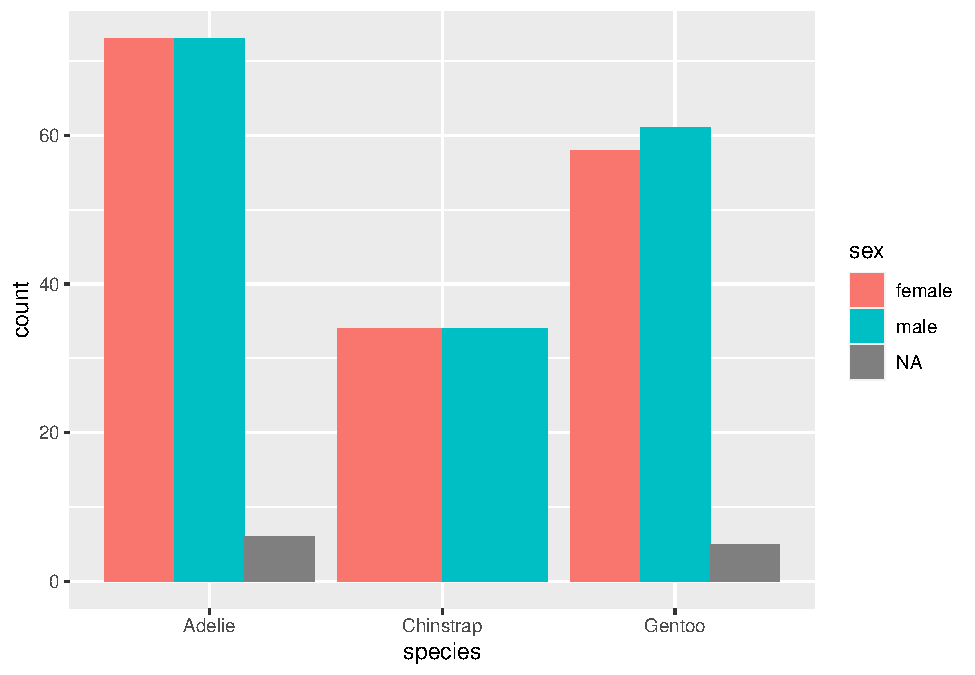
\includegraphics{intro_stats_files/figure-latex/unnamed-chunk-61-1.pdf}

This graph does correctly show that the sexes are pretty much equally balances across all three species.

\hypertarget{exercise-8a}{%
\paragraph*{Exercise 8(a)}\label{exercise-8a}}
\addcontentsline{toc}{paragraph}{Exercise 8(a)}

Using \texttt{species} and \texttt{island}, create a side-by-side bar chart. Be careful, though, to change the sample code above to make sure \texttt{species} is now the response variable (using the \texttt{fill} aesthetic) and that \texttt{island} is the explanatory variable (using \texttt{x}). (Hey, that's another hint to go back and look at the previous exercise and make sure you got part (a) right!)

\begin{Shaded}
\begin{Highlighting}[]
\CommentTok{\# Add code here to make a side{-}by{-}side bar chart.}
\end{Highlighting}
\end{Shaded}

\hypertarget{exercise-8b}{%
\paragraph*{Exercise 8(b)}\label{exercise-8b}}
\addcontentsline{toc}{paragraph}{Exercise 8(b)}

Comment on the association or independence of the two variables.

Please write up your answer here.

\hypertarget{categorical-recoding}{%
\section{Recoding factor variables}\label{categorical-recoding}}

As mentioned earlier, there are situations where a categorical variable is not recorded in R as a factor variable. Let's look at the \texttt{year} variable:

\begin{Shaded}
\begin{Highlighting}[]
\FunctionTok{glimpse}\NormalTok{(penguins}\SpecialCharTok{$}\NormalTok{year)}
\end{Highlighting}
\end{Shaded}

\begin{verbatim}
##  int [1:344] 2007 2007 2007 2007 2007 2007 2007 2007 2007 2007 ...
\end{verbatim}

These appear as integers. Yes, years are whole numbers, but why might this variable be treated as categorical data and not numerical data?

\hypertarget{exercise-9a}{%
\paragraph*{Exercise 9(a)}\label{exercise-9a}}
\addcontentsline{toc}{paragraph}{Exercise 9(a)}

Use the \texttt{tabyl} command to create a frequency table for \texttt{year}.

\begin{Shaded}
\begin{Highlighting}[]
\CommentTok{\# Add code here to make a frequency table for year.}
\end{Highlighting}
\end{Shaded}

\hypertarget{exercise-9b}{%
\paragraph*{Exercise 9(b)}\label{exercise-9b}}
\addcontentsline{toc}{paragraph}{Exercise 9(b)}

Why is \texttt{year} better thought of as categorical data and not numerical data (at least for this data set---we're not claiming years should always be treated as categorical)?

Please write up your answer here.

\begin{center}\rule{0.5\linewidth}{0.5pt}\end{center}

While the \texttt{tabyl} command seemed to work just fine with the \texttt{year} data in integer format, there are other commands that will not work so well. For example, \texttt{ggplot} often fails to do the right thing when a categorical variable is coded as a number. Therefore, we need a way to change numerically coded variables to factors.

The code below uses a command called \texttt{mutate} that takes an old variable and creates a new variable. (You'll learn more about this command in a later chapter. For now, you can just copy and paste this code if you need it again.) The name of the new variable can be anything we want; we'll just call it \texttt{year\_fct}. Then the real work is being done by the \texttt{as\_factor} command that concerts the numeric \texttt{year} variable into a factor variable.

Observe the effect below:

\begin{Shaded}
\begin{Highlighting}[]
\NormalTok{penguins }\OtherTok{\textless{}{-}}\NormalTok{ penguins }\SpecialCharTok{\%\textgreater{}\%}
    \FunctionTok{mutate}\NormalTok{(}\AttributeTok{year\_fct =} \FunctionTok{as\_factor}\NormalTok{(year))}
\FunctionTok{glimpse}\NormalTok{(penguins)}
\end{Highlighting}
\end{Shaded}

\begin{verbatim}
## Rows: 344
## Columns: 9
## $ species           <fct> Adelie, Adelie, Adelie, Adelie, Adelie, Adelie, Adel~
## $ island            <fct> Torgersen, Torgersen, Torgersen, Torgersen, Torgerse~
## $ bill_length_mm    <dbl> 39.1, 39.5, 40.3, NA, 36.7, 39.3, 38.9, 39.2, 34.1, ~
## $ bill_depth_mm     <dbl> 18.7, 17.4, 18.0, NA, 19.3, 20.6, 17.8, 19.6, 18.1, ~
## $ flipper_length_mm <int> 181, 186, 195, NA, 193, 190, 181, 195, 193, 190, 186~
## $ body_mass_g       <int> 3750, 3800, 3250, NA, 3450, 3650, 3625, 4675, 3475, ~
## $ sex               <fct> male, female, female, NA, female, male, female, male~
## $ year              <int> 2007, 2007, 2007, 2007, 2007, 2007, 2007, 2007, 2007~
## $ year_fct          <fct> 2007, 2007, 2007, 2007, 2007, 2007, 2007, 2007, 2007~
\end{verbatim}

\hypertarget{exercise-10a}{%
\paragraph*{Exercise 10(a)}\label{exercise-10a}}
\addcontentsline{toc}{paragraph}{Exercise 10(a)}

Make a contingency table of the species measured in each year using counts. Use the \texttt{species} variable first, followed by the new factor variable \texttt{year\_fct}. (Think about why that order makes sense. \textbf{We will always list the response variable first so that the categories of interest will be the rows and the groups will be the columns.})

\begin{Shaded}
\begin{Highlighting}[]
\CommentTok{\# Add code here to make a contingency table for species and year with counts.}
\end{Highlighting}
\end{Shaded}

\hypertarget{exercise-10b}{%
\paragraph*{Exercise 10(b)}\label{exercise-10b}}
\addcontentsline{toc}{paragraph}{Exercise 10(b)}

Make a contingency table of the species measured in each year using column percentages (\emph{not} proportions). (Again, be sure to use the new factor variable \texttt{year\_fct}, not the old variable \texttt{year}.)

\begin{Shaded}
\begin{Highlighting}[]
\CommentTok{\# Add code here to make a contingency table for species and year with percentages.}
\end{Highlighting}
\end{Shaded}

\hypertarget{exercise-10c}{%
\paragraph*{Exercise 10(c)}\label{exercise-10c}}
\addcontentsline{toc}{paragraph}{Exercise 10(c)}

How similar or dissimilar are the distributions of species across the three years of the study?

Please write up your answer here.

\hypertarget{categorical-pub}{%
\section{Publication-ready graphics}\label{categorical-pub}}

Let's go back to the first relative frequency bar chart from this chapter.

\begin{Shaded}
\begin{Highlighting}[]
\FunctionTok{ggplot}\NormalTok{(penguins, }\FunctionTok{aes}\NormalTok{(}\AttributeTok{x =}\NormalTok{ species, }\AttributeTok{y =}\NormalTok{ ..prop.., }\AttributeTok{group =} \DecValTok{1}\NormalTok{)) }\SpecialCharTok{+}
    \FunctionTok{geom\_bar}\NormalTok{()}
\end{Highlighting}
\end{Shaded}

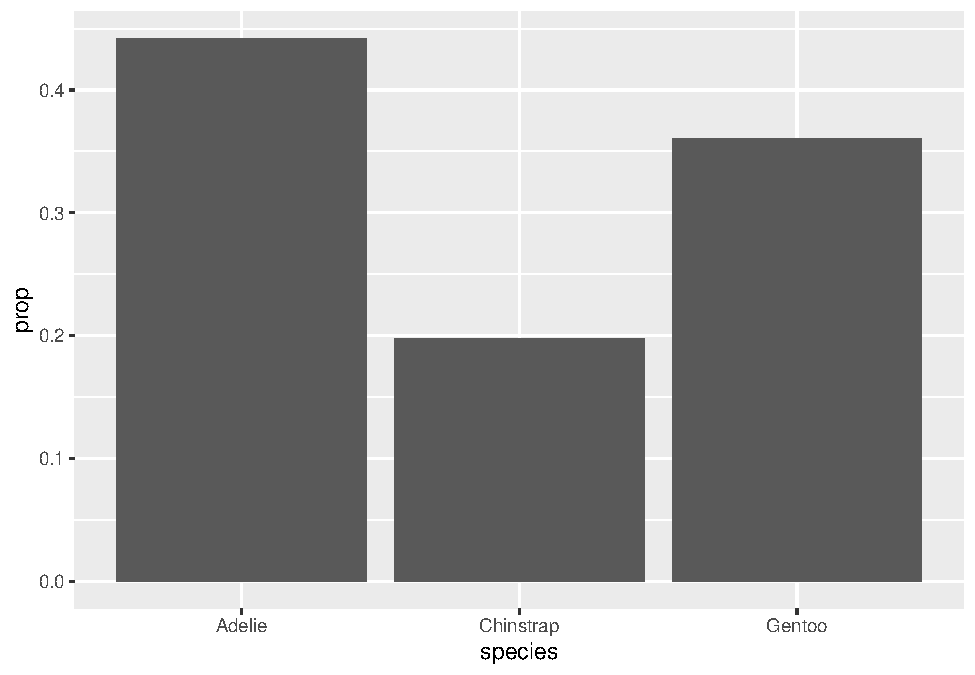
\includegraphics{intro_stats_files/figure-latex/unnamed-chunk-68-1.pdf}

The variable name \texttt{species} is already informative, but the y-axis is labeled with ``prop''. Also note that this graph could use a title. We can do all this with \texttt{labs} (for labels). Observe:

\begin{Shaded}
\begin{Highlighting}[]
\FunctionTok{ggplot}\NormalTok{(penguins, }\FunctionTok{aes}\NormalTok{(}\AttributeTok{x =}\NormalTok{ species, }\AttributeTok{y =}\NormalTok{ ..prop.., }\AttributeTok{group =} \DecValTok{1}\NormalTok{)) }\SpecialCharTok{+}
    \FunctionTok{geom\_bar}\NormalTok{() }\SpecialCharTok{+}
    \FunctionTok{labs}\NormalTok{(}\AttributeTok{title =} \StringTok{"Distribution of species"}\NormalTok{,}
         \AttributeTok{y =} \StringTok{"Proportion"}\NormalTok{,}
         \AttributeTok{x =} \StringTok{"Species"}\NormalTok{)}
\end{Highlighting}
\end{Shaded}

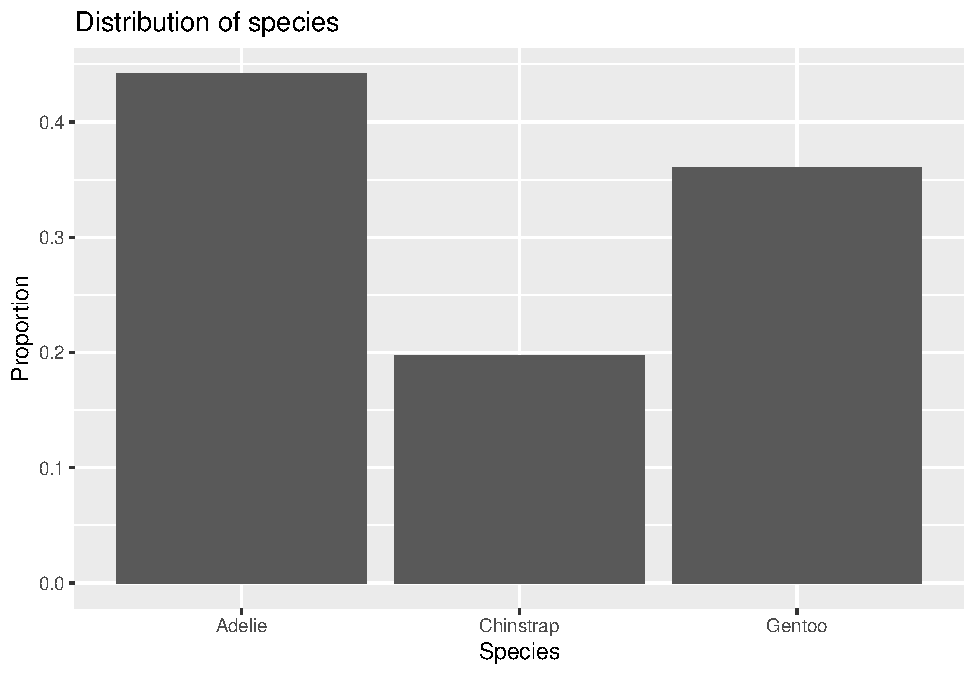
\includegraphics{intro_stats_files/figure-latex/unnamed-chunk-69-1.pdf}

\hypertarget{exercise-11}{%
\paragraph*{Exercise 11}\label{exercise-11}}
\addcontentsline{toc}{paragraph}{Exercise 11}

Modify the following side-by-side bar chart by adding a title and labels for both the fill variable and the x-axis variable. (Hint: you can use \texttt{fill\ =\ sex} inside the \texttt{labs} command just like you used \texttt{title}, \texttt{y}, and \texttt{x}.)

\begin{Shaded}
\begin{Highlighting}[]
\CommentTok{\# Modify the following side{-}by{-}side bar chart by adding a title and }
\CommentTok{\# labels for both the x{-}axis and the fill variable.}
\FunctionTok{ggplot}\NormalTok{(penguins, }\FunctionTok{aes}\NormalTok{(}\AttributeTok{fill =}\NormalTok{ sex, }\AttributeTok{x =}\NormalTok{ species)) }\SpecialCharTok{+}
    \FunctionTok{geom\_bar}\NormalTok{(}\AttributeTok{position =} \StringTok{"dodge"}\NormalTok{)}
\end{Highlighting}
\end{Shaded}

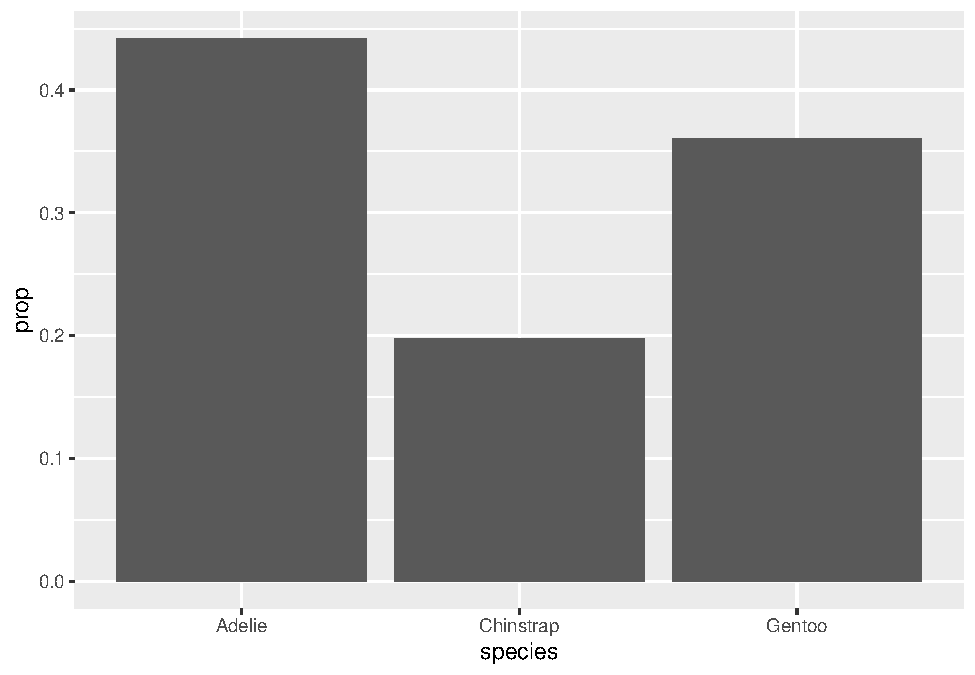
\includegraphics{intro_stats_files/figure-latex/unnamed-chunk-70-1.pdf}

\hypertarget{categorical-summary}{%
\section{Plotting summary data}\label{categorical-summary}}

Everything we did above was summarizing \emph{raw data}; that is, the data consisted of all the observations for each individual penguin. Often, though, when you find data out in the wild, that data will be summarized into a table already and you may not have access to the raw data.

For example, let's suppose that you found some data online, but it looked like this:

\begin{longtable}[]{@{}ll@{}}
\toprule()
species & count \\
\midrule()
\endhead
Adelie & 152 \\
Chinstrap & 68 \\
Gentoo & 124 \\
\bottomrule()
\end{longtable}

This raises two questions:

\begin{enumerate}
\def\labelenumi{\arabic{enumi}.}
\tightlist
\item
  How would you get this data into R?
\item
  How would you plot the data?
\end{enumerate}

To answer the first question, we show you how to create your own tibble. Here is the syntax:

\begin{Shaded}
\begin{Highlighting}[]
\NormalTok{penguin\_species\_table }\OtherTok{\textless{}{-}} \FunctionTok{tibble}\NormalTok{(}
    \AttributeTok{species =} \FunctionTok{c}\NormalTok{(}\StringTok{"Adelie"}\NormalTok{, }\StringTok{"Chinstrap"}\NormalTok{, }\StringTok{"Gentoo"}\NormalTok{),}
    \AttributeTok{count =} \FunctionTok{c}\NormalTok{(}\DecValTok{152}\NormalTok{, }\DecValTok{68}\NormalTok{, }\DecValTok{124}\NormalTok{)}
\NormalTok{)}
\NormalTok{penguin\_species\_table}
\end{Highlighting}
\end{Shaded}

\begin{verbatim}
## # A tibble: 3 x 2
##   species   count
##   <chr>     <dbl>
## 1 Adelie      152
## 2 Chinstrap    68
## 3 Gentoo      124
\end{verbatim}

Basically, the \texttt{tibble} command creates a new tibble. Then each column of data must be entered manually as a ``vector'' using the \texttt{c} to group all the data values together for each column. Be careful about the placement of quotation marks, commas, and parentheses.

Once we have our summary data, we want to make a bar chart. But this won't work:

\begin{Shaded}
\begin{Highlighting}[]
\FunctionTok{ggplot}\NormalTok{(penguin\_species\_table, }\FunctionTok{aes}\NormalTok{(}\AttributeTok{x =}\NormalTok{ species)) }\SpecialCharTok{+}
    \FunctionTok{geom\_bar}\NormalTok{()}
\end{Highlighting}
\end{Shaded}

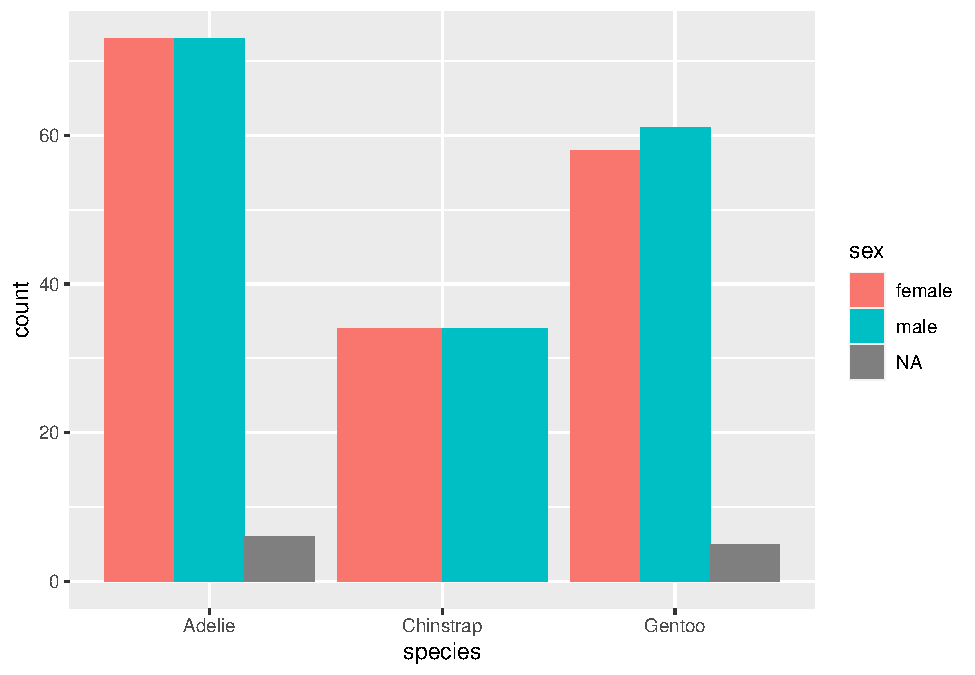
\includegraphics{intro_stats_files/figure-latex/unnamed-chunk-72-1.pdf}

\hypertarget{exercise-12}{%
\paragraph*{Exercise 12}\label{exercise-12}}
\addcontentsline{toc}{paragraph}{Exercise 12}

Explain what went wrong with the previous command? Why does \texttt{ggplot} think that each species has count 1?

Please write up your answer here.

\begin{center}\rule{0.5\linewidth}{0.5pt}\end{center}

Instead, we need to use \texttt{geom\_col}. This works a lot like \texttt{geom\_bar} except that it also requires a \texttt{y} value in its aesthetics to force the command to look for the counts in some other variable in the data.

\begin{Shaded}
\begin{Highlighting}[]
\FunctionTok{ggplot}\NormalTok{(penguin\_species\_table, }\FunctionTok{aes}\NormalTok{(}\AttributeTok{x =}\NormalTok{ species, }\AttributeTok{y =}\NormalTok{ count)) }\SpecialCharTok{+}
    \FunctionTok{geom\_col}\NormalTok{()}
\end{Highlighting}
\end{Shaded}

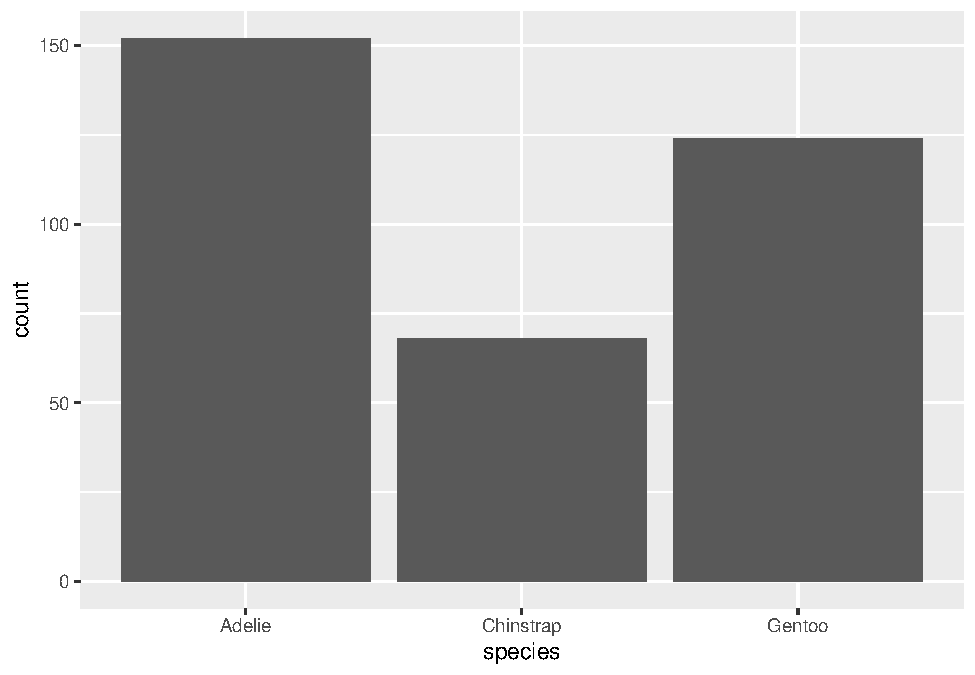
\includegraphics{intro_stats_files/figure-latex/unnamed-chunk-73-1.pdf}

\hypertarget{exercise-13a}{%
\paragraph*{Exercise 13(a)}\label{exercise-13a}}
\addcontentsline{toc}{paragraph}{Exercise 13(a)}

Use the \texttt{tabyl} command to create a frequency table for \texttt{island}.

\begin{Shaded}
\begin{Highlighting}[]
\CommentTok{\# Add code here to create a frequency table for island}
\end{Highlighting}
\end{Shaded}

\hypertarget{exercise-13b}{%
\paragraph*{Exercise 13(b)}\label{exercise-13b}}
\addcontentsline{toc}{paragraph}{Exercise 13(b)}

Use the \texttt{tibble} command to create a new tibble manually that contains the frequency data for the \texttt{island} variable. It should have two columns, one called \texttt{island} and the other called \texttt{count}. Name it \texttt{penguin\_island\_table}.

\begin{Shaded}
\begin{Highlighting}[]
\CommentTok{\# Add code here to create a tibble with frequency data for island}
\end{Highlighting}
\end{Shaded}

\hypertarget{exercise-13c}{%
\paragraph*{Exercise 13(c)}\label{exercise-13c}}
\addcontentsline{toc}{paragraph}{Exercise 13(c)}

Use \texttt{ggplot} with \texttt{geom\_col} to create a bar chart for island.

\begin{Shaded}
\begin{Highlighting}[]
\CommentTok{\# Add code here to create a bar chart for island}
\end{Highlighting}
\end{Shaded}

\hypertarget{categorical-conclusion}{%
\section{Conclusion}\label{categorical-conclusion}}

You can summarize a single categorical variable using a frequency table. For only one categorical variable, a graph is usually overkill, but if you really want a graph, the bar chart is the best option. Both raw counts and proportions/percentages can be useful.

We use contingency tables to summarize two categorical variables. Unless groups are of equal size, raw counts can be incredibly misleading here. You should include proportions/percentages to be able to compare the distributions across groups. If the proportions/percentages are roughly the same, the variables are more likely to be independent, whereas if the proportions/percentages are different, there may be an association between the variables. For graphing, the best choice is usually a side-by-side bar chart. A stacked bar chart will also work, especially if using relative frequencies on the y-axis, but it can be hard to compare across groups when the response variable has three or more categories.

Sometimes we come across categorical data that is recorded using numbers. Many R commands will not work properly if they expect factors and receive numbers, so we use the \texttt{mutate} command to create a new variable along with \texttt{as\_factor} to convert the numbers to categories.

Sometimes we come across summary data instead of raw data. We can then manually create tibbles with that summary data and use \texttt{geom\_col} instead of \texttt{geom\_bar} to graph it.

\hypertarget{categorical-prep}{%
\section{Preparing and submitting your assignment}\label{categorical-prep}}

\begin{enumerate}
\def\labelenumi{\arabic{enumi}.}
\tightlist
\item
  From the ``Run'' menu, select ``Restart R and Run All Chunks''.
\item
  Deal with any code errors that crop up. Repeat steps 1---2 until there are no more code errors.
\item
  Spell check your document by clicking the icon with ``ABC'' and a check mark.
\item
  Hit the ``Preview'' button one last time to generate the final draft of the \texttt{.nb.html} file.
\item
  Proofread the HTML file carefully. If there are errors, go back and fix them, then repeat steps 1--5 again.
\end{enumerate}

If you have completed this chapter as part of a statistics course, follow the directions you receive from your professor to submit your assignment.

  \bibliography{book.bib,packages.bib}

\end{document}
